\documentclass[a4paper,12pt,oneside]{report}
\usepackage{OvidiusFMI}

\usepackage{times}
\usepackage{graphicx}
\usepackage{hyperref}
\usepackage{color,xcolor}
\usepackage{framed}
\usepackage{enumerate}
\usepackage{listings}
\usepackage{amsmath,amsfonts,amssymb,amsthm,epsfig,epstopdf,url,array}
\usepackage{multicol,multirow}
%\usepackage{xspace}
%\include{command}
\definecolor{code}{rgb}{0.97,0.97,0.97}
\lstdefinestyle{customc}{
  belowcaptionskip=1\baselineskip,
  backgroundcolor=\color{code},
  breaklines=true,
%  frame=L,
%  xleftmargin=\parindent,
  language=C,
  showstringspaces=false,
  morekeywords={bool,
  				 glutMainLoop, glutIdleFunc, glMatrixMode, glLoadIdentity, glPushMatrix, glPopMatrix, 
  				 glBegin, glEnd, glTranslatef, glRotatef, glScalef, glColor3f, glColor4f, glutSolidCube, glutWireCube, glutSolidSphere,
  				 glutWireSphere, glutSolidCone,glutSetWindowTitle,glutGet,glClear,glutSwapBuffers,glDepthFunc,
  				 glutWireCone, glutSolidTorus, glutWireTorus, glutSolidDodecahedron, glutWireDodecahedron,
  				 glutSolidOctahedron, glutWireOctahedron, glutSolidTetrahedron, glutWireTetrahedron, 
  				 glVertex3f,glVertex2f,glPointSize,
  				 glutSolidIcosahedron, glutWireIcosahedron, glutSolidTeapot, glutWireTeapot,glutReshapeFunc,
  				 glFlush, gluPerspective, glutPostRedisplay, glutInit, glutKeyboardFunc,glutKeyboardUpFunc,
  				 glutInitWindowSize, glutInitWindowPosition, glutInitDisplayMode, glutCreateWindow, glutDisplayFunc,glutPassiveMotionFunc,
  				 glClear,glTexCoord2f,
  				 glEnable, glDisable, glLightfv, glMaterialfv, glCullFace,glViewport,
  				 glFrontFace,glColor3ub, glShadeModel,
  				 glGenLists, glGetFloatv,glGentextures,glTexImage2D,glTexParameteri, free, glDeleteTextures,
  				 glLineStipple, glLineWidth, glBindTexture,glGenTextures,
  				 glNewList, glEndList, glCallList,
  				 glMap1f,glEvalCoord1f,glMapGrid1d,glEvalMesh1,glMap2f,glEvalCoord2f,glMapGrid2f,glEvalMesh2,
  				 gluBeginTrim, gluEndTrim, gluPwlCurve,glHint,
  				 GLUnurbsObj, gluBeginSurface, gluNurbsSurface, gluEndSurface, gluNewNurbsRenderer, 									gluNurbsProperty,gluQuadricNormals,
  				 glNormal3f,
  				 gluQuadricTexture,GLUquadricObj,gluSphere,
  				 glPolygonMode, glBlendFunc,glFogi,glFogiv,glFogfv,
  				 GLfloat, GLdouble, GLint,GLuint, GLushort,GLubyte, glRasterPos2f,
  				 gluBeginCurve, gluNurbsCurve, gluEndCurve,
  				 glOrtho, gluLookAt, glutBitmapCharacter, 
  				 glInitNames, glPushName, glLoadName, glSelectBuffer, glRenderMode,gluPickMatrix, glGetIntegerv, glutMouseFunc,glutMotionFunc,system,
  				 glPushAttrib, glPopAttrib, glMultMatrixf, sprintf, glClearStencil, glStencilFunc,glStencilOp,glStencilMask,glColorMask,glActiveStencilFaceEXT,fprintf},  
%   numbers=left,                    % where to put the line-numbers; possible values are (none, left, right)
  %numbersep=5pt,                   % how far the line-numbers are from the code
  %numberstyle=\tiny\color{code}, % the style that is used for the line-numbers
  basicstyle=\footnotesize\ttfamily,
  keywordstyle=\bfseries\color{green!40!black},
  commentstyle=\itshape\color{purple!40!black},
  identifierstyle=\color{blue},
  stringstyle=\color{orange},
}

\lstset{escapechar=@,style=customc}

%\makeindex
% Remove command to get current date 

%-----------------------------------------------------------------------------------------------------------%
% START - PORTIUNE CUSTOMIZABILA PRIMA PAGINA DE CATRE FIECARE ABSOLVENT%
%vvvvvvvvvvvvvvvvvvvvvvvvvvvvvvvvvvvvvvvvvvvvvvvvvvvvvvvvvvvvvvvvvvvvvvvvvvv%

\facultatea{Matematic\u a \c si Informatic\u a}

%decomentati specializarea corespunzatoare domeniului si comentati ce nu corespunde
\specializarea{Informatic\u a}
%\specializare{Matematic\u a}
%\specializare{Matematic\u a - Informatic\u a}

%decomentati tipul lucrarii de absolvire si comentati ce nu corespunde
\teza{licen\c t\u a}
%\teza{diserta\c tie}

\titlu{Aplica\c tie pentru organizarea \c si gestionarea evenimentelor}

% Orice lucrare are cel putin un coordonator stiintific. Primul este OBLIGATORIU si il vom 
% numi Coordonator Principal
\gradDidacticCP{Lect. univ. dr.}%OBLIGATORIU
\coordonatorPrincipal{Rusu Andrei} %OBLIGATORIU
% Daca exista doi coordonatori se va preciza si cel de al doilea
%\gradDidacticCS{Asist. univ. dr.} %OPTIONAL
%\coordonatorSecundar{Nume Prenume Coordonator Secundar} %OPTIONAL

\autor{Ene Luis Adrian}
\data{2026}% anul sustinerii lucrarii

%^^^^^^^^^^^^^^^^^^^^^^^^^^^^^^^^^^^^^^^^^^^^^^^^^%
% END - PORTIUNE CUSTOMIZABILA PRIMA PAGINA DE CATRE FIECARE ABSOLVENT%
%---------------------------------------------------------------------------------------------------------%

\begin{document}
\maketitle

\pagenumbering{roman}
\tableofcontents
\listoffigures

\pagenumbering{arabic}

%\include{prefata} % OPTIONAL
%\include{multumiri} % OPTIONAL

\chapter*{Rezumat}
\addcontentsline{toc}{chapter}{Rezumat}

Lucrarea de licen\c t\u a \emph{Aplica\c tie web pentru organizarea \c si gestionarea evenimentelor} propune dezvoltarea unei platforme complete destinate organizatorilor \c si participan\c tilor la conferin\c te, meeting-uri, concerte, evenimente culturale \c si, \^intr-o m\u asur\u a mai mic\u a, competi\c tii sportive. Aplica\c tia (implementare: proiectul ManFast) permite publicarea evenimentelor, filtrarea dup\u a nume, jude\c t \c si dat\u a, achizi\c tionarea biletelor nominale cu plat\u a online prin Stripe \c si administrarea participan\c tilor printr-un panou dedicat.

Solu\c tia tehnic\u a adopt\u a arhitectura client-server: frontend React 19 cu Material UI 9, backend Node.js/Express, baz\u a de date PostgreSQL. Autentificarea utilizeaz\u a token-uri JWT, parole hash-uite cu bcrypt, verificare email la \^inregistrare (cod de 6 cifre) \c si resetare parol\u a. Administratorii gestioneaz\u a evenimente (inclusiv imagini), efectueaz\u a check-in \c si promoveaz\u a al\c ti administratori.

Documentul prezint\u a motiva\c tia temei, starea domeniului, proiectarea \c si implementarea solu\c tiei, capturi din aplica\c tia func\c tional\u a \c si concluzii. Platforma reprezint\u a o solu\c tie scalabil\u a, adaptabil\u a contextului rom\^anesc (pl\u a\c ti RON, jude\c te).

\textbf{Cuvinte cheie}: aplicație web, gestionarea evenimentelor, bilete digitale, plată online, autentificare securizată.

\vspace{1cm}
\chapter*{Abstract}
\addcontentsline{toc}{chapter}{Abstract}

The bachelor's thesis Web application for organizing and managing events proposes the development of a complete platform for organizers and participants in conferences, meetings, concerts, cultural events, and to a lesser extent sports competitions. The application (implementation: ManFast project) enables event publishing, filtering by name, county and date, purchasing nominal tickets with online payment via Stripe, and participant management through a dedicated admin panel.

The technical solution adopts a client-server architecture: React 19 frontend with Material UI 9, Node.js/Express backend, PostgreSQL database. Authentication uses JWT tokens, bcrypt password hashing, email verification on registration (6-digit code), and password reset. Administrators manage events (including images), perform check-in, and promote other administrators.

The document presents the motivation, domain state, solution design and implementation, application screenshots, and conclusions. The platform represents a scalable solution adapted to the Romanian context (RON payments, counties).

\textbf{Keywords}: web application, event management, digital tickets, online payment, secure authentication.

\clearpage
\chapter{Motiva\c tie}
\sloppy


\section{Contextul \c si problema}

Organizarea \textbf{conferin\c telor, meeting-urilor, concertelor} \c si a altor evenimente cu public \c si locuri limitate implic\u a, \^in mod tradi\c tional, procese fragmentate: promovarea prin canale diferite (re\c tele sociale, email, site-uri proprii), v\^anzarea biletelor sau \^inscrierilor \^in format fizic sau prin transfer bancar manual, \c si validarea participan\c tilor la intrare prin liste pe h\^artie. Aceast\u a abordare genereaz\u a erori, pierderi de timp \c si dificult\u a\c ti \^in reconcilierea pl\u a\c tilor cu locurile rezervate.

Digitalizarea procesului — centralizarea informa\c tiilor despre evenimente, automatizarea pl\u a\c tilor \c si asocierea fiec\u arui bilet cu identitatea participantului — reprezint\u a un pas natural \^in contextul extinderii serviciilor online \c si al a\c stept\u arilor utilizatorilor privind comoditatea \c si securitatea tranzac\c tiilor \cite{fielding2000, stripe2024}.

Organizatorii (universit\u a\c ti, firme, asocia\c tii culturale, s\u ali de concert) nu dispun adesea de resurse pentru solu\c tii enterprise costisitoare. \^In acela\c si timp, platformele interna\c tionale generice nu sunt \^intotdeauna adaptate pie\c tei locale: moneda RON, structura administrativ\u a pe jude\c te, sau necesitatea unui flux simplu de check-in administrat de organizator. Pentru \textbf{evenimente sportive} amatoriale, acelea\c si mecanisme (\^inscriere, plat\u a, list\u a nominal\u a) sunt utile, dar reprezint\u a un caz secundar fa\c t\u a de conferin\c te \c si concerte.

Participan\c tii au nevoie de o interfa\c t\u a clar\u a: descoperire evenimente, filtrare, achizi\c tia rapid\u a a unuia sau  a mai multor bilete nominale, vizualizarea istoricului \c si gestionarea contului. Organizatorii au nevoie de un panou unic pentru publicare, monitorizare locuri disponibile \c si confirmare prezen\c t\u a la fa\c ta locului.




\section{Obiectivele lucr\u arii}

Obiectivul principal este proiectarea \c si implementarea \textbf{Aplica\c tiei web pentru organizarea \c si gestionarea evenimentelor}, care s\u a \^indeplineasc\u a urm\u atoarele obiective specifice:

\begin{enumerate}
	\item Implementarea unui modul de autentificare securizat: \^inregistrarea cu verificarea e-mailului, login JWT, resetarea parolei, editarea profilului \c si \c stergerea contului.
	\item Oferirea unei interfe\c te publice pentru listarea evenimentelor viitoare, cu filtre dup\u a nume, jude\c t \c si dat\u a.
	\item Permiterea achizi\c tion\u arii biletelor nominale (unul sau mai multe nume per tranzac\c tie) cu plat\u a online prin Stripe Checkout, \^in moneda RON.
	\item Dezvoltarea unui panou de administrare pentru CRUD evenimente (inclusiv imagini), list\u a participan\c ti \c si check-in.
	\item Gestionarea rolurilor utilizator/admin \c si promovarea/revocarea administratorilor cu parol\u a de autorizare.
	\item Documentarea arhitecturii, a modelului de date \c si a fluxurilor principale (UML, ERD).
\end{enumerate}

Lucrarea demonstreaz\u a integrarea tehnologiilor web moderne \^intr-un produs coerent, testabil \c si prezentabil, cu respectarea unor practici de securitate recunoscute \cite{fowler2002}.


\section{Structura documentului}

Prezenta lucrare este organizat\u a structural pe capitole, dup\u a cum urmeaz\u a:

\vspace{0.2cm}
\begin{description}
	\setlength{\itemsep}{0.3cm}
	\item[Capitolul 2] Analizeaz\u a \^in detaliu starea actual\u a a domeniului. Cuprinde studii relevante din literatur\u a, o analiz\u a a platformelor existente pe pia\c t\u a \c si o compara\c tie direct\u a cu solu\c tia propus\u a.
	\item[Capitolul 3] Descrie \^in profunzime arhitectura sistemului \c si detaliile de implementare ale aplica\c tiei. Sunt incluse cerin\c tele func\c tionale \c si non-func\c tionale, tehnologiile alese, diagramele UML, structura bazei de date \c si fragmente de cod surs\u a relevante.
	\item[Capitolul 4] Prezint\u a interfe\c tele grafice ale aplica\c tiei prin intermediul unor capturi de ecran detaliate, mapate pe fluxurile principale de utilizare.
	\item[Capitolul 5] Sintetizeaz\u a concluziile generale ale proiectului, eviden\c tiaz\u a limit\u arile identificate pe parcursul dezvolt\u arii \c si propune viitoarele direc\c tii de dezvoltare.
\end{description}


\section{Tipuri de evenimente vizate}
\sloppy
Aplica\c tia web pentru organizarea \c si gestionarea evenimentelor este conceput\u a \^in jurul unor formate frecvente \^in via\c ta academic\u a, cultural\u a \c si profesional\u a. \textit{Tabelul 1.1} sintetizeaz\u a ca-tegoriile principale, actorii implica\c ti \c si modul \^in care platforma le sus\c tine. 

\begin{table}[htbp]
	\centering
	\renewcommand{\arraystretch}{1.5} 
	\setlength{\tabcolsep}{10pt} %	
	\begin{tabular}{|l|l|p{5.5cm}|} 
		\hline
		\textbf{Tip Eveniment} & \textbf{Actori Principali} & \textbf{Scenariu \^in Aplica\c tie} \\ \hline
		Conferin\c t\u a / Meeting & Organizator, Participant & Publicare cu detalii complete (dat\u a, locuri limitate, descriere, pre\c t \^in RON), \^inregistrare online \c si check-in la intrare. \\ \hline
		Concert / Festival & Organizator, Public & Accent pe componenta vizual\u a (galerie de imagini), redirec\c tionare rapid\u a c\u atre Stripe Checkout pentru achizi\c tie bilet nominal. \\ \hline
		Competi\c tie Sportiv\u a & Admin, Sportiv & \^Inscriere pe baz\u a de bilet nominal, check-in realizat de organizator la \^inregistrarea \^in concurs (caz secundar). \\ \hline
	\end{tabular}

	\caption{Tipuri de evenimente reflectate \^in aplica\c tie}
	\label{tab:evenimente}
\end{table}

\subsection{Conferin\c te, meeting-uri \c si evenimente profesionale}

Universit\u a\c ti, camere de comer\c t \c si firme de consultan\c t\u a organizeaz\u a periodic conferin\c te \c si meeting-uri cu num\u ar limitat de locuri. Participan\c tii trebuie s\u a se \^inregistreze, s\u a-\c si confirme identitatea (email verificat) \c si, uneori, s\u a achite o tax\u a de participare. Platforma acoper\u a acest flux end-to-end: publicarea evenimentului cu dat\u a, loca\c tie (jude\c t, localitate) \c si capacitate, urmat\u a de \^inregistrare online \c si emitere bilet nominal.

Pentru meeting-uri interne sau seminarii pl\u atite, administratorul poate crea evenimente cu pre\c t fix \c si num\u ar redus de locuri; sistemul decrementeaz\u a automat locurile disponibile la fiecare tranzac\c tie confirmat\u a. Check-in-ul din panoul admin permite validarea prezen\c tei la recep\c tie sau la intrarea \^in sal\u a util at\^at pentru conferin\c te, c\^at \c si pentru training-uri corporate.

\subsection{Concerte \c si evenimente culturale}

Concertele \c si festivalurile locale necesit\u a o prezentare atractiv\u a (titlu, descriere, mai multe imagini) \c si v\^anzare rapid\u a a biletelor. Aplica\c tia permite \^inc\u arcarea a p\^an\u a la opt imagini per eveniment, afi\c sarea galeriei pe pagina de detalii \c si redirect c\u atre Stripe Checkout pentru plat\u a securizat\u a.

\newpage Filtrarea dup\u a jude\c t \c si dat\u a ajut\u a publicul s\u a descopere evenimente din apropiere relevant pentru turnee na\c tionale de concerte sau festivaluri itinerante. Biletele nominale asigur\u a c\u a fiecare loc este asociat unui participant, reduc\^and rev\^anzarea neautorizat\u a \c si simplific\^and controlul la intrare.

\subsection{Evenimente sportive \c si utilizare complementar\u a}

Modelul actual al aplica\c tiei (nume pe bilet, check-in administrat manual) se preteaz\u a \c si competi\c tiilor sportive amatoriale sau turneelor locale, unde organizatorul trebuie s\u a verifice identitatea participantului. Aceast\u a ni\c s\u a este secundar\u a fa\c t\u a de conferin\c te, concerte \c si meeting-uri: nu sunt implementate func\c tionalit\u a\c ti specifice sportului (categorii de v\^arst\u a, echipe, program meciuri), dar fluxul general de \^inscriere \c si plat\u a r\u am\^ane valabil.

Extinderi viitoare (categorii de bilete, abonamente de sezon) ar putea \^int\u ari suportul sportiv f\u ar\u a a modifica arhitectura de baz\u a.

\subsection{ Beneficii transversale}



Indiferent de tipul evenimentului, organizatorul beneficiaz\u a de: 

\begin{itemize}
	\item \textbf{Un singur panou} pentru toate formatele: nu este nevoie de solu\c tii separate pentru conferin\c te vs. concerte.
	\item \textbf{Trasabilitate pl\u a\c ti}: fiecare bilet este legat de o sesiune Stripe \c si de un utilizator a-utentificat.
	\item \textbf{Adaptare local\u a}: jude\c te rom\^ane\c sti, moned\u a RON, e-mailuri prin SMTP Brevo.
	\item \textbf{Control asupra datelor}: baza PostgreSQL self-hosted, f\u ar\u a dependen\c t\u a de un marketplace global.
\end{itemize}

\vspace{1em} % Spa\c tiu \^intre list\u a \c si urm\u atorul paragraf

Aceast\u a diversitate de cazuri de utilizare justific\u a alegerea unui model de date simplu (eveniment unic, pre\c t unic, bilete nominale) care r\u am\^ane suficient de expresiv pentru majoritatea scenariilor \^int\^alnite. % OBLIGATORIU
\chapter{Starea actual\u a a domeniului}
\vspace*{-1cm}
\^In acest capitol este analizat contextul \^in care se \^incadreaz\u a aplica\c tia web pentru organizarea \c si gestionarea evenimentelor: cercet\u ari relevante pentru comer\c tul electronic, ticketing online \c si securitate web, platforme existente \c si o compara\c tie func\c tional\u a.

\section{Studii \c si articole \c stiin\c tifice}

\subsection{Arhitecturi web \c si API-uri REST}

Fielding \cite{fielding2000} define\c ste principiile REST (\textit{Representational State Transfer}) ca stil arhitectural pentru sisteme distribuite. Separarea clientului de server, utilizarea resurselor adresabile prin URI \c si a metodelor HTTP standard (GET, POST, PUT, DELETE) faciliteaz\u a dezvoltarea aplica\c tiilor web scalabile. ManFast expune un API REST \^in Node.js/Express, consumat de frontend-ul React abordare aliniat\u a cu recomand\u arile din literatura de specialitate.

Fowler \cite{fowler2002} descrie tipare de proiectare enterprise, inclusiv separarea responsabilit\u a\c tilor \^intre straturi (prezentare, logic\u a de business, persisten\c t\u a). Aplica\c tia analizat\u a respect\u a acest principiu: React gestioneaz\u a UI, Express con\c tine regulile de business, PostgreSQL stocheaz\u a datele.

\subsection{Securitatea autentific\u arii}

OWASP \cite{owasp2024} enumer\u a bune practici pentru autentificare: hash-uirea parolelor (nu stocarea \^in clar), protec\c tia sesiunilor, limitarea ratei de cereri, validarea input-ului. ManFast implementeaz\u a bcrypt pentru parole, JWT cu expirare 24h, rate limiting pe codurile de verificare a e-mailurilor \c si resetare parolei.

Standardul JWT (JSON Web Token) \cite{jwt2015} permite transmiterea securizat\u a a claims-urilor \^intre p\u ar\c ti. Token-ul semnat con\c tine id-ul utilizatorului \c si rolul (user/admin), verificat la fiecare cerere protejat\u a.

Provos \c si Mazi\`eres \cite{bcrypt1999} introduc bcrypt, algoritm de hash adaptat la cost computa\c tional configurabil, rezistent la atacuri brute-force pe parole. ManFast folose\c ste cost factor 10.

\subsection{Pl\u a\c ti online \c si gateway-uri}

Documenta\c tia Stripe \cite{stripe2024} descrie fluxul Checkout: sesiune de plat\u a g\u azduit\u a, redirect c\u atre pagina securizat\u a Stripe, confirmare prin webhook sau verificare sesiune. ManFast creeaz\u a sesiuni Checkout cu metadata (event\_id, user\_id, nume participan\c ti) \c si confirm\u a plata prin endpoint dedicat, f\u ar\u a a stoca date de card pe serverul propriu --- reduc\^and responsabilitatea PCI-DSS.

\subsection{Persisten\c t\u a \c si baze de date rela\c tionale}

PostgreSQL \cite{postgresql2024} ofer\u a tranzac\c tii ACID, constr\u angeri de integritate referen\c tial\u a \c si tipuri \linebreak avansate (ex.: array pentru imagini eveniment). Schema ManFast exploateaz\u a aceste capabilit\u a\c ti pentru consisten\c ta bilete/locuri disponibile.

\subsection{Interfa\c t\u a utilizator \c si SPA}

React \cite{react2024} \c si ecosistemul s\u au permit construirea de \textit{Single Page Applications reactive}. Material UI \cite{mui2024} ofer\u a componente accesibile \c si responsive. ManFast utilizeaz\u a React 19, Vite pentru build rapid \c si MUI 9 cu tem\u a dark personalizat\u a.

\section{Aplica\c tii dedicate domeniului}

\subsection{Eventbrite}

Eventbrite \cite{eventbrite2024} este o platform\u a interna\c tional\u a pentru crearea \c si promovarea evenimentelor, cu v\^anzare bilete, pagini de destina\c tie \c si instrumente de marketing. Ofer\u a check-in prin cod QR \c si analiz\u a audien\c t\u a. Platforma suport\u a multiple tipuri de evenimente: concerte, conferin\c te, workshop-uri. Fluxul tipic: organizatorul creeaz\u a pagina evenimentului, seteaz\u a pre\c turile \c si capacitatea, promoveaz\u a link-ul, iar participan\c tii achizi\c tioneaz\u a bilete online.

Limit\u ari pentru organizatori mici: comisioane per bilet, personalizare redus\u a a fluxului de check-in, dependen\c t\u a de ecosistemul proprietar. Datele participan\c tilor sunt stocate pe infrastructura Eventbrite, nu \^in controlul direct al organizatorului. Pentru conferin\c te cu sesiuni paralele sau concerte cu locuri numerotate, unele func\c tionalit\u a\c ti avansate pot lipsi sau necesit\u a addon-uri pl\u atite.

Din perspectiva tehnologic\u a, astfel de platforme folosesc arhitecturi cloud scalabile, procesare pl\u a\c ti prin PSP integrat \c si aplica\c tii mobile pentru scanare QR. ManFast adopt\u a un subset al acestor capabilit\u a\c ti, orientat spre simplitate \c si control local al datelor \^in PostgreSQL.




\subsection{Platforme locale \c si generice}

Pe pia\c ta rom\^aneasc\u a exist\u a solu\c tii pentru bilete la concerte \c si festivaluri (iaBilet, Eventim), precum \c si platforme e-commerce generice (WooCommerce, Shopify) care pot vinde ``produse'' reprezent\^and locuri la eveniment. Acestea sunt optimizate pentru v\^anzare la scar\u a larg\u a, nu neap\u arat pentru meeting-uri corporate sau conferin\c te universitare.

Organizatorii locali folosesc frecvent formulare Google, pl\u a\c ti directe \c si liste Excel solu\c tii cu cost zero ini\c tial, dar cu risc ridicat de erori \c si lips\u a de audit trail pentru pl\u a\c ti. Reconcilierea manual\u a a listei de participan\c ti cu transferurile bancare consum\u a timp \c si poate genera dispute la intrarea \^in sal\u a.

Aplica\c tia propus\u a \^incerc\u a s\u a ofere un echilibru: cost de operare redus (self-hosted), flux clar de la descoperire eveniment la plat\u a \c si check-in, f\u ar\u a complexitatea unei platforme glo-bale. Adaptarea la jude\c tele rom\^ane\c ti \c si pl\u a\c ti RON via Stripe reprezint\u a un avantaj competitiv \^in contextul local fa\c t\u a de solu\c tiile generice interna\c tionale.

\subsection{Tendin\c te \c si standarde \^in industria ticketing-ului}

Industria biletelor electronice a crescut accelerat dup\u a pandemia COVID-19, c\^and contactless check-in \c si pl\u a\c tile online au devenit norm\u a. Platformele mature investesc \^in trei direc\c tii: (1) experien\c t\u a mobil\u a — aplica\c tii native sau PWA pentru scanare rapid\u a; (2) analitic\u a — dashboard-uri de v\^anz\u ari, heatmap-uri de pre\c turi dinamice; (3) integrare marketing — email automation, remarketing pe re\c tele sociale.

ManFast nu urm\u are\c ste replicarea tuturor acestor capabilit\u a\c ti enterprise, ci func\c tionalitatea minim\u a viabil\u a pentru organizatori locali: publicare eveniment, v\^anzare online, list\u a \linebreak participan\c ti, check-in la intrare. Aceast\u a decizie de scope este aliniat\u a cu principiul MVP (\textit{Minimum Viable Product}) din literatura de product management.

\subsection{Conformitate PCI-DSS \c si delegarea pl\u a\c tilor}

Standardul PCI-DSS (\textit{Payment Card Industry Data Security Standard}) impune m\u asuri stricte pentru orice sistem care proceseaz\u a, stocheaz\u a sau transmite date de card. Solu\c tiile care folosesc Stripe Checkout hosted deleg\u a colectarea datelor sensibile c\u atre Stripe comerciantul prime\c ste doar confirmarea pl\u a\c tii prin API. \newpage ManFast adopt\u a explicit acest model: frontend-ul redirec\c tioneaz\u a utilizatorul pe domeniul \textbf{checkout.stripe.com}, iar backend-ul verific\u a statusul sesiunii f\u ar\u a a vedea num\u arul de card.

Aceast\u a abordare reduce suprafa\c ta de atac \c si simplific\u a auditul de securitate pentru o lucrare de licen\c t\u a, men\c tin\^and totodat\u a un flux profesional de plat\u a recunoscut de utilizatori.

\subsection{Arhitectura SPA \c si API REST}

Aplica\c tiile \textit{Single Page Application} (SPA) [8] \^incarc\u a o singur\u a pagin\u a HTML \c si navigheaz\u a prin JavaScript, ob\c tin\^and date de la server prin API JSON.

 \textbf{Avantaje}: interfa\c t\u a reactiv\u a, separare clar\u a frontend/backend, posibilitatea de a extinde ulterior cu aplica\c tie mobil\u a consum\^and acela\c si API.

\textbf{Dezavantaje} relevante pentru ManFast: SEO limitat pe pagini dinamice (acceptabil pentru platform\u a cu autentificare), necesitatea gestion\u arii token-ului JWT pe client. Compara\c tia cu arhitectura server-side rendering (Next.js) ar fi o extensie viitoare; pentru licen\c t\u a, Vite + React ofer\u a timp de dezvoltare redus \c si ecosistem bogat (Material UI).

\subsection{Studiu de caz: fluxul utilizatorului \^in platforme consacrate}

Pe Eventbrite, utilizatorul parcurge: descoperire eveniment → selectare tip bilet → checkout → email confirmare cu PDF/QR. Organizatorul acceseaz\u a dashboard cu statistici v\^anz\u ari \c si export CSV participan\c ti.

ManFast simplific\u a acest flux pentru organizatori locali (conferin\c te, concerte, meeting-uri):

- un singur tip de bilet pe eveniment (pre\c t unic);

- nume nominal obligatoriu (identificare la check-in);

- f\u ar\u a marketplace global, evenimentele sunt listate doar pe instan\c ta ManFast;

- check-in manual din panou admin, f\u ar\u a aplica\c tie mobil\u a dedicat\u a scan\u arii QR (extensie viitoare).

Aceast\u a simplificare reduce complexitatea implement\u arii \c si timpul de \^inv\u a\c tare pentru administratori neexperimenta\c ti \^in IT.

\section{Criterii de evaluare a solu\c tiilor}

Pentru a fundamenta compara\c tia din \textit{Tabelul 2.2}, au fost definite criterii ponderate:

Adecvare func\c tional\u a (40\%) — suport bilete nominale, check-in, filtrare local\u a.

Cost total de operare (20\%) — comisioane PSP, abonamente platform\u a, hosting.

Control date (20\%) — unde sunt stocate datele participan\c tilor, export, GDPR.

Personalizare (10\%) — posibilitatea modific\u arii fluxului sau branding.

Securitate autentificare (10\%) — verificare email, reset parol\u a, roluri.

ManFast ob\c tine scor ridicat la control date \c si personalizare (cod deschis, PostgreSQL propriu), scor mediu la cost (Stripe per tranzac\c tie, hosting self-managed), \c si scor bun la adecvare func\c tional\u a pentru ni\c sa aleas\u a.

Aceste analize suplimentare contextualizeaz\u a pozi\c tionarea ManFast fa\c t\u a de solu\c tiile \newline  existente \c si justific\u a alegerile de scope ale proiectului.

\section{Analiz\u a comparativ\u a}

Tabelul~\ref{tab:comparatie} sintetizeaz\u a diferen\c tele \^intre platforme reprezentative \c si aplica\c tia propus\u a.

\begin{table}[htbp]
	\centering
	\renewcommand{\arraystretch}{1.5} 
	\setlength{\tabcolsep}{6pt} 
	\begin{tabular}{|>{\raggedright\arraybackslash}p{3.5cm}|>{\raggedright\arraybackslash}p{2.2cm}|>{\raggedright\arraybackslash}p{2.5cm}|>{\raggedright\arraybackslash}p{3.5cm}|}
		\hline
		\textbf{Func\c tionalitate} & \textbf{Eventbrite} & \textbf{Generic e-comm} & \textbf{Aplica\c tia propus\u a} \\ \hline
		Bilete nominale & Da & Par\c tial & Da \\ \hline
		Pl\u a\c ti Stripe RON & Nu (alte PSP) & Variabil & Da \\ \hline
		Check-in admin & Da (QR) & Nu & Da (list\u a) \\ \hline
		Verificare email register & Da & Variabil & Da (cod 6 cifre) \\ \hline
		Filtrare jude\c t/dat\u a & Da & Nu & Da (42 jude\c te) \\ \hline
		Cod deschis / personalizabil & Nu & Nu & Da \\ \hline
		Reset parol\u a tel.+email & Variabil & Variabil & Da \\ \hline
	\end{tabular}
	\caption{Compara\c tie func\c tional\u a}
	\label{tab:comparatie}
\end{table}

\section{Concluzii par\c tiale}

Analiza demonstreaz\u a c\u a exist\u a un spa\c tiu pentru o solu\c tie adaptat\u a: conferin\c te, meeting-uri, concerte \c si evenimente culturale, cu pl\u a\c ti RON via Stripe, bilete pe nume \c si admi-nistrare simpl\u a. Aplica\c tia propune o implementare open-source, extensibil\u a, care integreaz\u a func\c tionalit\u a\c tile esen\c tiale \c si le aliniaz\u a cu cerin\c tele locale (jude\c te, SMTP Brevo pentru e-mailuri).

\vspace{0.3cm}
\noindent Urm\u atorul capitol detaliaz\u a arhitectura, tehnologiile \c si implementarea solu\c tiei propuse. % OBLIGATORIU
\chapter{Solu\c tia propus\u a}

\vspace*{-1cm}
\section{Cerin\c te func\c tionale pentru utilizator \c si \newline nefunc\c tionale}

\subsection{Cerin\c te func\c tionale pentru utilizator}

\begin{itemize}
	\item \textbf{RF-U1} --- \^Inregistrare cont: username, email, telefon, parol\u a; trimitere cod 6 cifre pe email; creare cont dup\u a verificare.
	\item \textbf{RF-U2} --- Autentificare cu email \c si parol\u a; primire token JWT.
	\item \textbf{RF-U3} --- Resetare parol\u a prin email sau telefon (email mascat la c\u autare dup\u a telefon).
	\item \textbf{RF-U4} --- Vizualizare list\u a evenimente viitoare; filtre: nume, jude\c t, dat\u a.
	\item \textbf{RF-U5} --- Pagin\u a detalii eveniment: descriere, imagini, loca\c tie, pre\c t, locuri.
	\item \textbf{RF-U6} --- Cump\u arare bilete nominale (1..N nume); redirect Stripe Checkout.
	\item \textbf{RF-U7} --- Confirmare plat\u a; vizualizare bilete \^in ``Biletele mele'' (viitoare/trecute).
	\item \textbf{RF-U8} --- Editare profil; schimbare parol\u a; \c stergere cont (cu confirmare parol\u a).
\end{itemize}

\subsection{Cerin\c te func\c tionale pentru administrator}

\begin{itemize}
	\item \textbf{RF-A1} --- CRUD evenimente: titlu, descriere, dat\u a, jude\c t, localitate, loca\c tie, pre\c t, locuri, durat\u a, imagini (max 8).
	\item \textbf{RF-A2} --- List\u a participan\c ti per eveniment; check-in.
	\item \textbf{RF-A3} --- Promovare/revocare rol admin (cu parol\u a autorizare); protec\c tie ultim admin.
\end{itemize}

\subsection{Cerin\c te nefunc\c tionale}

\begin{itemize}
	\item \textbf{RNF-1 Securitate} --- bcrypt, JWT, hash token-uri/coduri, CORS, rate limiting.
	\item \textbf{RNF-2 Disponibilitate} --- API stateless; DB rela\c tional\u a.
	\item \textbf{RNF-3 UX} --- Responsive; tem\u a dark; mesaje eroare clare.
	\item \textbf{RNF-4 Mentenabilitate} --- Separare frontend/backend; migr\u ari SQL.
	\item \textbf{RNF-5 Portabilitate} --- Node.js 18+, PostgreSQL 14+.
\end{itemize}

\section{Arhitectura sistemului}

ManFast urmeaz\u a arhitectura \textbf{client-server} \^in trei straturi:

\begin{enumerate}
	\item \textbf{Strat prezentare} --- SPA React (Vite), routing React Router, context autentificare, apeluri \texttt{fetch} c\u atre API.
	\item \textbf{Strat aplica\c tie} --- Express: rute \texttt{/api/auth}, \texttt{/api/events}, \texttt{/api/tickets}; middleware JWT \c si \texttt{requireAdmin}.
	\item \textbf{Strat date} --- PostgreSQL; fi\c siere statice imagini \^in \texttt{uploads/}.
\end{enumerate}

Servicii externe: \textbf{Stripe} (pl\u a\c ti), \textbf{Brevo SMTP} (email verificare \c si reset).


\begin{figure}[htbp]
	\centering
	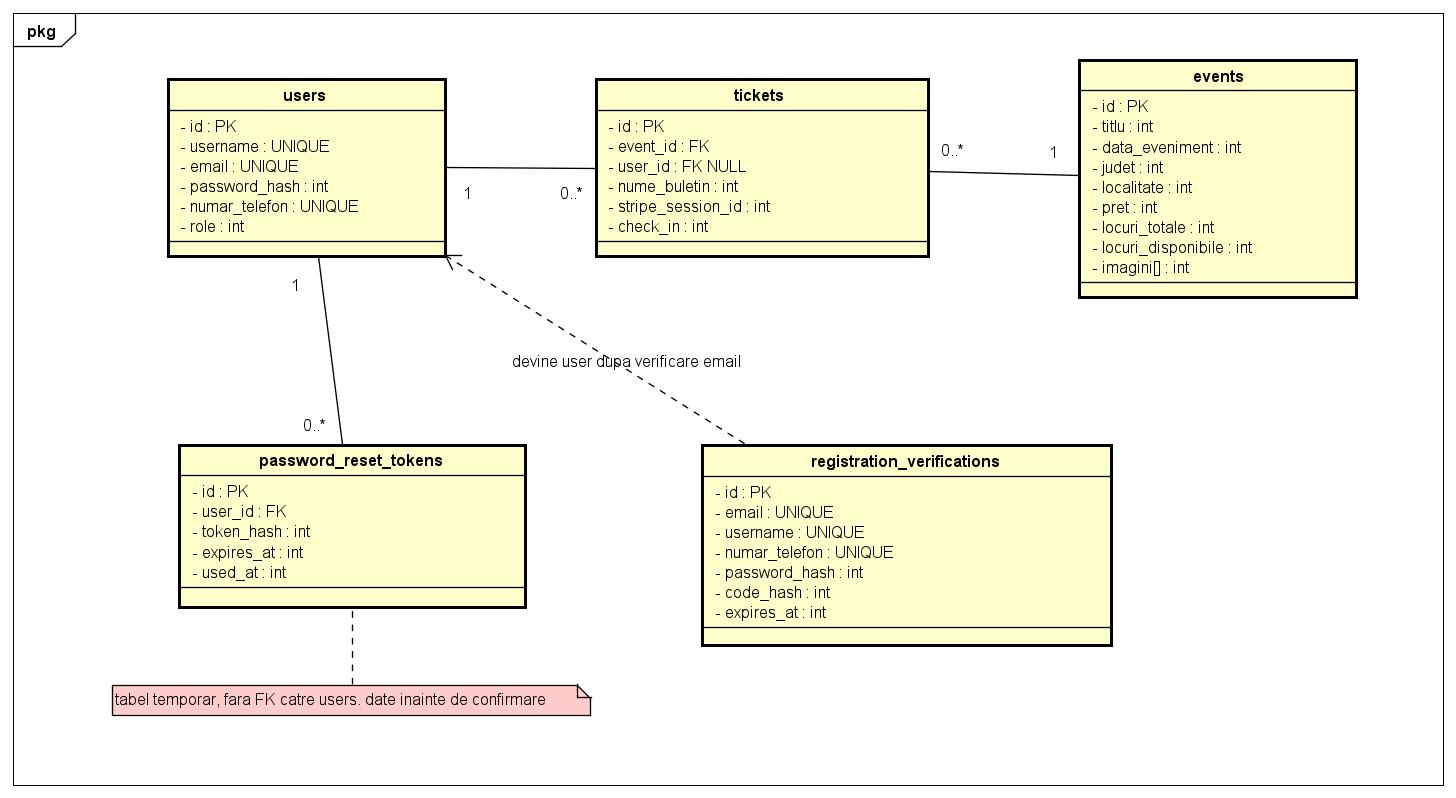
\includegraphics[width=1\textwidth]{Model de domeniu _ ERD ManFast.jpg}
	\caption{Arhitectura sistemului ManFast}
	\label{fig:l2f1}
\end{figure}

Instruc\c tiuni inserare: Diagrama blocuri: Browser (React+MUI) -> HTTPS/JSON -> Express API -> PostgreSQL; lateral Stripe \c si Brevo SMTP. Tool: draw.io, Lucidchart sau PowerPoint. Export PNG 300dpi, l\u a\c time ~14cm \^in document.


\section{Tehnologii utilizate}

\begin{table}[htbp]
	\centering
	\begin{tabular}{|l|p{8cm}|}
		\hline
		\textbf{Tehnologie} & \textbf{Rol} \\
		\hline
		React 19 + Vite 8 & Frontend SPA, HMR dev \\
		\hline
		Material UI 9 & Componente UI, tem\u a dark \\
		\hline
		Express 4 & API REST, Multer upload \\
		\hline
		PostgreSQL & Persisten\c t\u a rela\c tional\u a \\
		\hline
		JWT + bcrypt & Auth \c si hash parole \\
		\hline
		Stripe Checkout & Pl\u a\c ti card RON \\
		\hline
		Nodemailer + Brevo & Email SMTP \\
		\hline
	\end{tabular}
	\caption{Stack tehnologic ManFast}
	\label{tab:tech}
\end{table}

React [8] gestioneaz\u a starea UI \c si re-renderarea eficient\u a. Vite ofer\u a build rapid. Express [11] ruteaz\u a cererile HTTP. pg conecteaz\u a la PostgreSQL. Stripe SDK creeaz\u a sesiuni Checkout.

\section{Diagrame UML}
\subsection{Cazuri de utilizare}

Actorii principali sunt Utilizatorul (autentificat sau nu) \c si Administratorul. Utilizatorul
poate \^inregistra cont, autentifica, filtra evenimente, cump\u ara bilete, gestiona profilul. Administratorul public\u a evenimente, face check-in, gestioneaz\u a al\c ti admini. 

\begin{figure}[htbp]
	\centering
	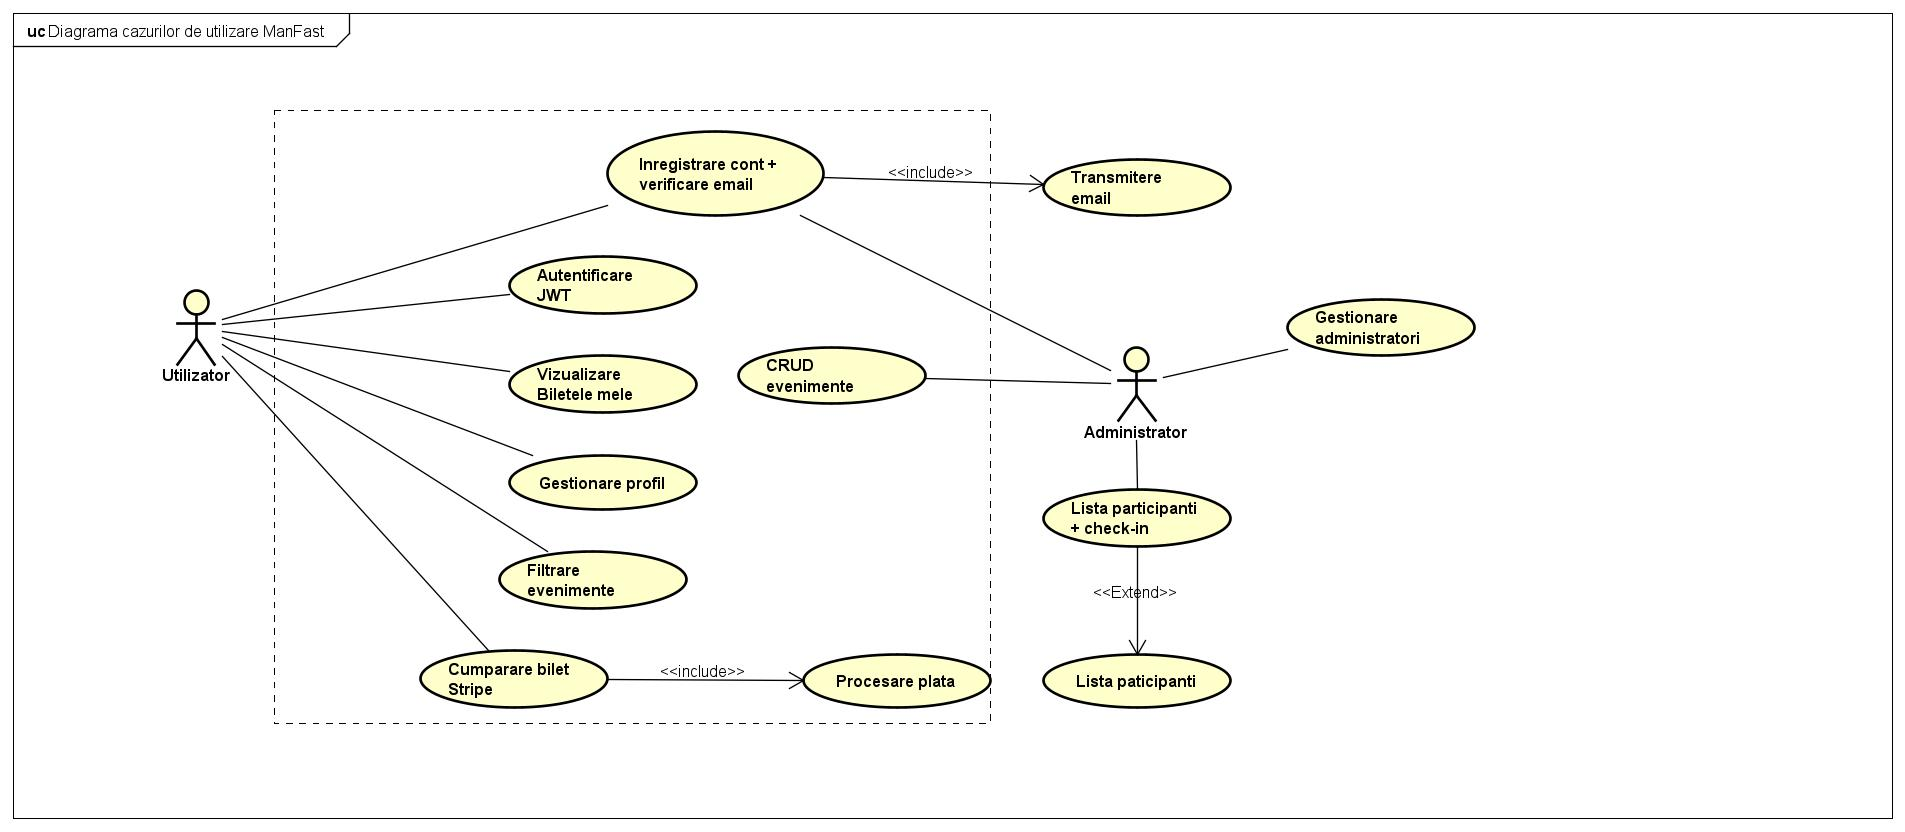
\includegraphics[width=1\textwidth]{Diagrama cazurilor de utilizare ManFast.jpg}
	\caption{ Diagrama cazurilor de utilizare}
	\label{fig:l2f1}
\end{figure}

Instruc\c tiuni inserare: UML use case: actor Utilizator (register, login, filtre, cump\u ar\u a bilet, profil); actor Admin (CRUD eveniment, check-in, promovare admin). Tool: StarUML, draw.io. Include sistem boundary ``ManFast''.

\subsection{Secven\c ta de \^inregistrare cu verificare prin email}

Flux: Frontend POST /register-> Backend valideaz\u a, salveaz\u a \^in \linebreak \texttt{registration\_verifications},
trimite cod SMTP -> Frontend POST /register/verify -> INSERT \texttt{users}.

\begin{figure}[htbp]
	\centering
	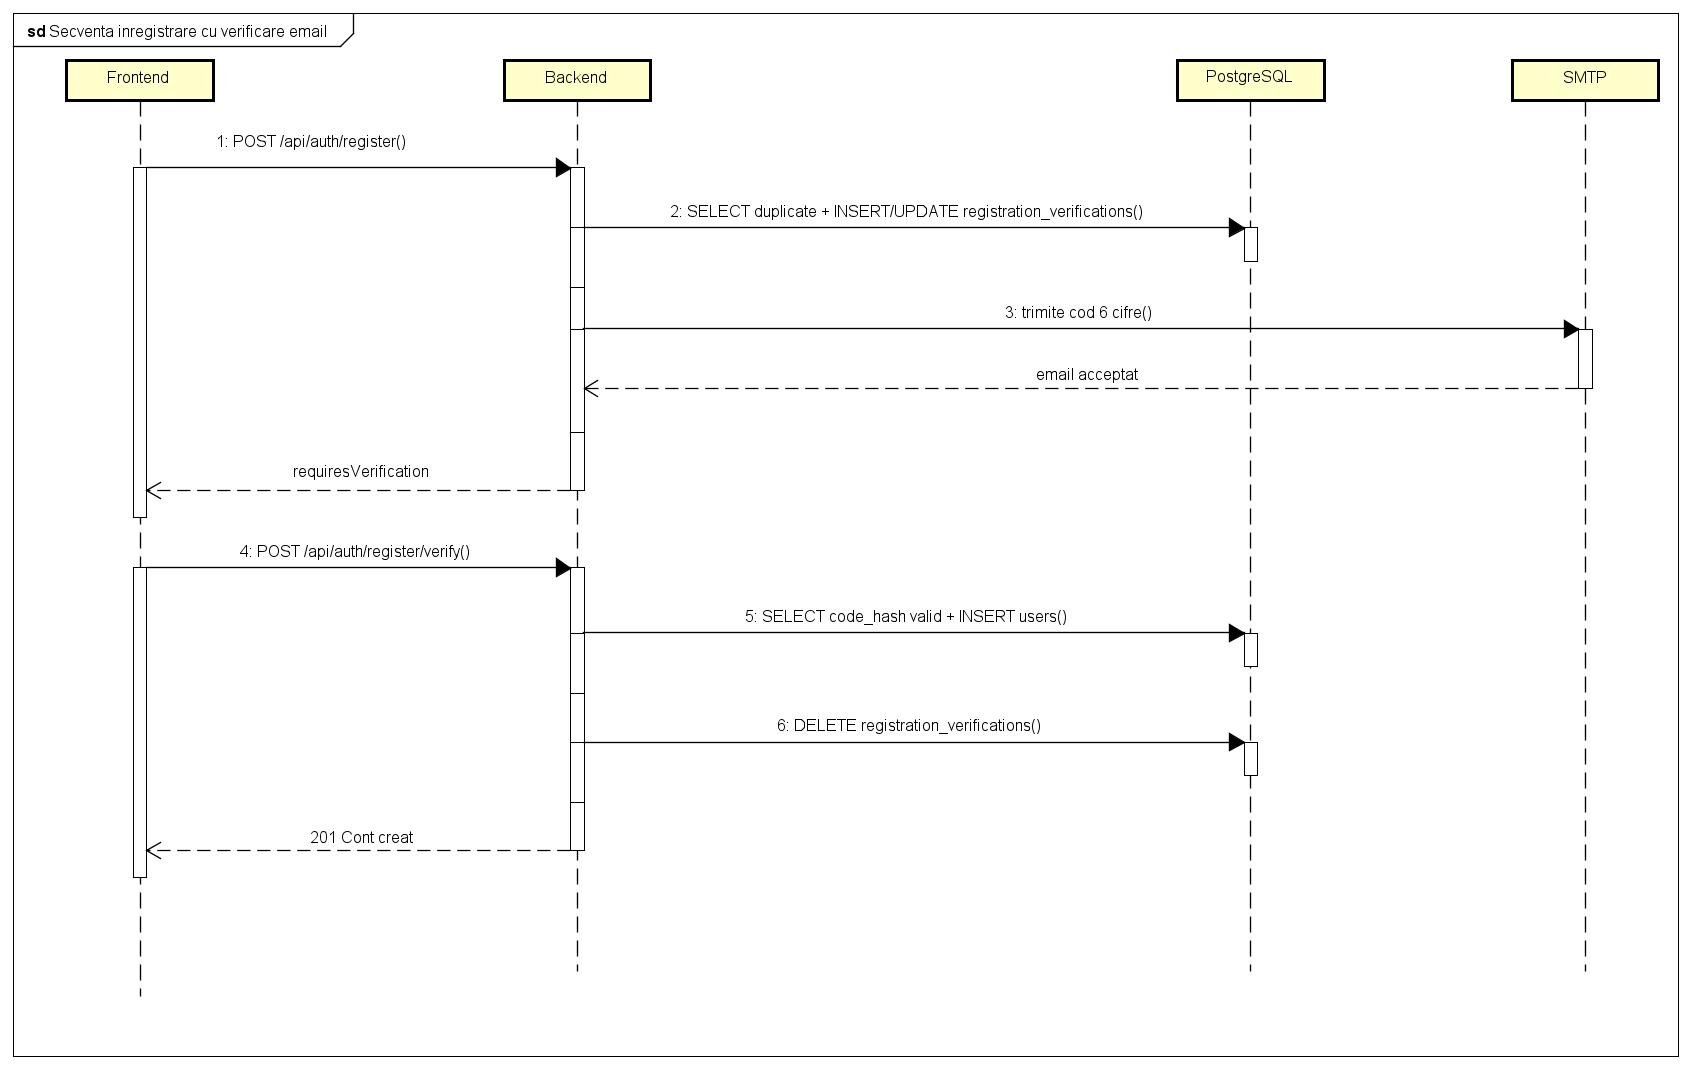
\includegraphics[width=1\textwidth]{Secventa inregistrare cu verificare email.jpg}
	\caption{Diagrama de secven\c t\u a - \^inregistrarea cu email}
	\label{fig:l2f1}
\end{figure}

Instruc\c tiuni inserare: Participan\c ti: Utilizator, Frontend, Backend, PostgreSQL, SMTP. Mesaje:
register, salveaz\u a temp, trimite cod, verify, creare user. Nota\c tii pe fiecare s\u ageat\u a.

\subsection{Secven\c ta pentru plata prin Stripe}

Flux: Frontend POST create-checkout-session -> redirect Stripe -> success URL -> confirm-payment -> INSERT tickets, UPDATE locuri.

Instruc\c tiuni inserare: Participan\c ti: Utilizator, Frontend, Backend, Stripe, DB. Include metadata session \c si confirm-payment.

\begin{figure}[htbp]
	\centering
	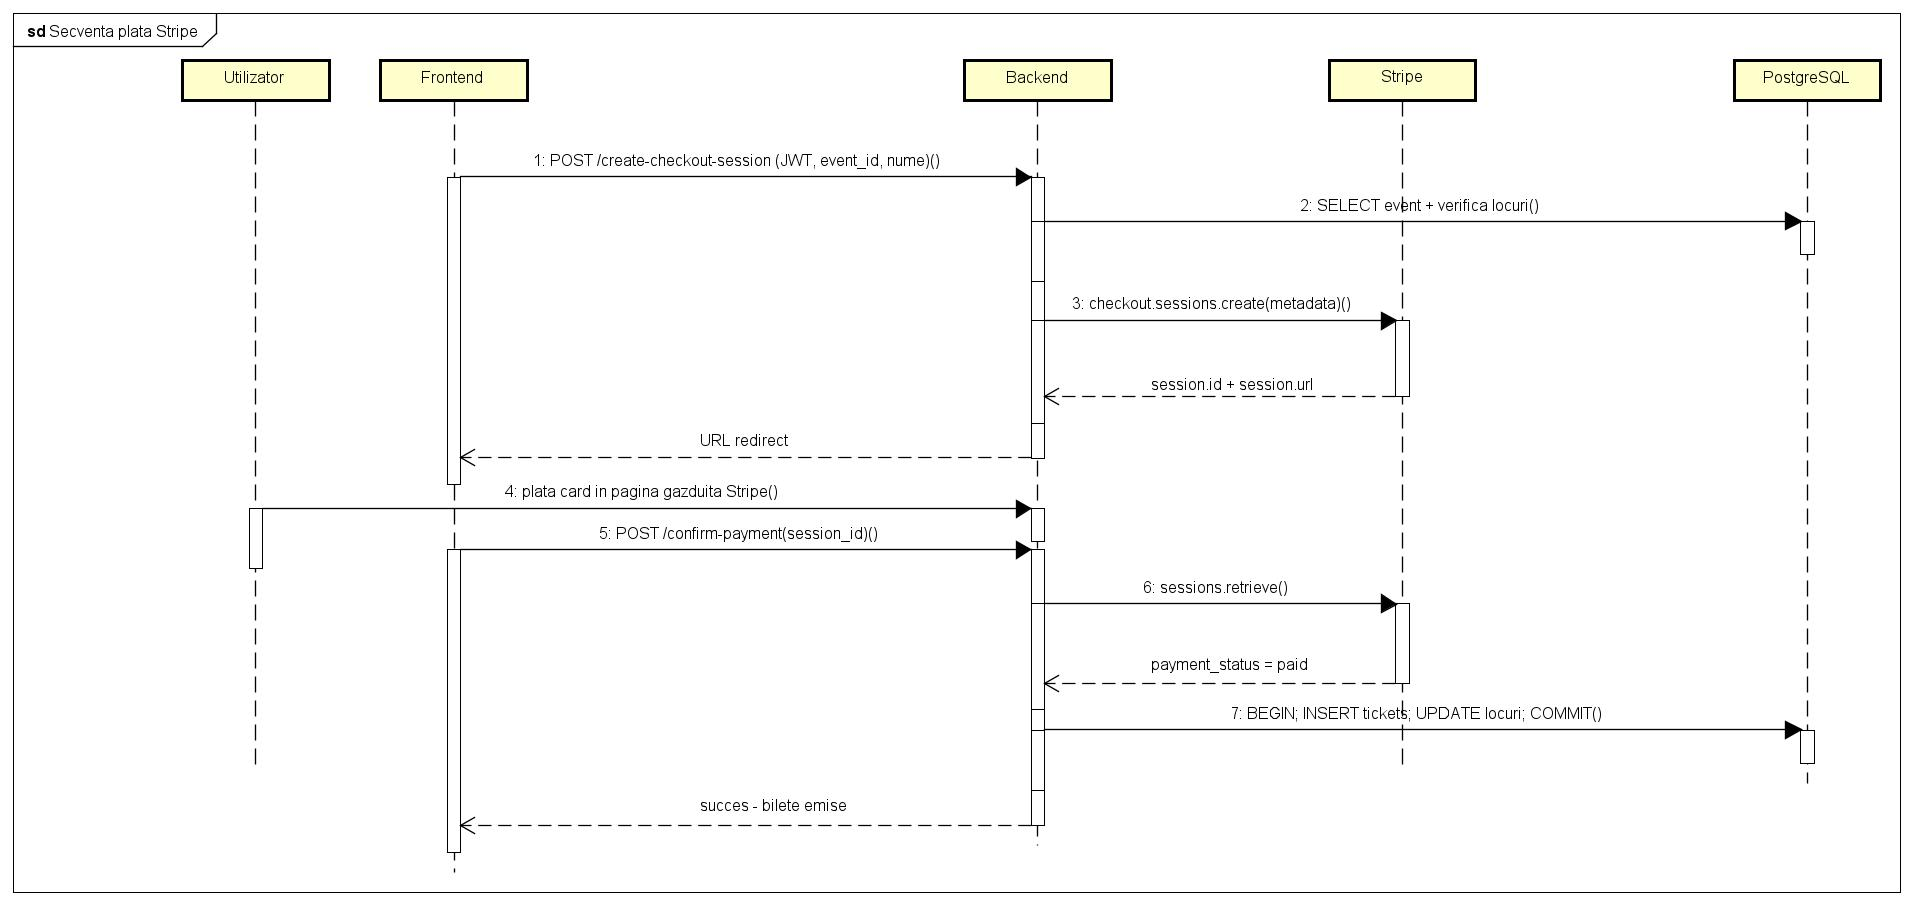
\includegraphics[width=1\textwidth]{Secventa plata Stripe.jpg}
	\caption{Diagrama de secven\c t\u a - plata Stripe}
	\label{fig:l2f1}
\end{figure}


\subsection{Activitatea la check-in \c si admin}

Instruc\c tiuni inserare: Flowchart: admin selecteaz\u a eveniment -> list\u a participan\c ti -> validare bilet -> UPDATE check\_in=true sau mesaj eroare

\begin{figure}[htbp]
	\centering
	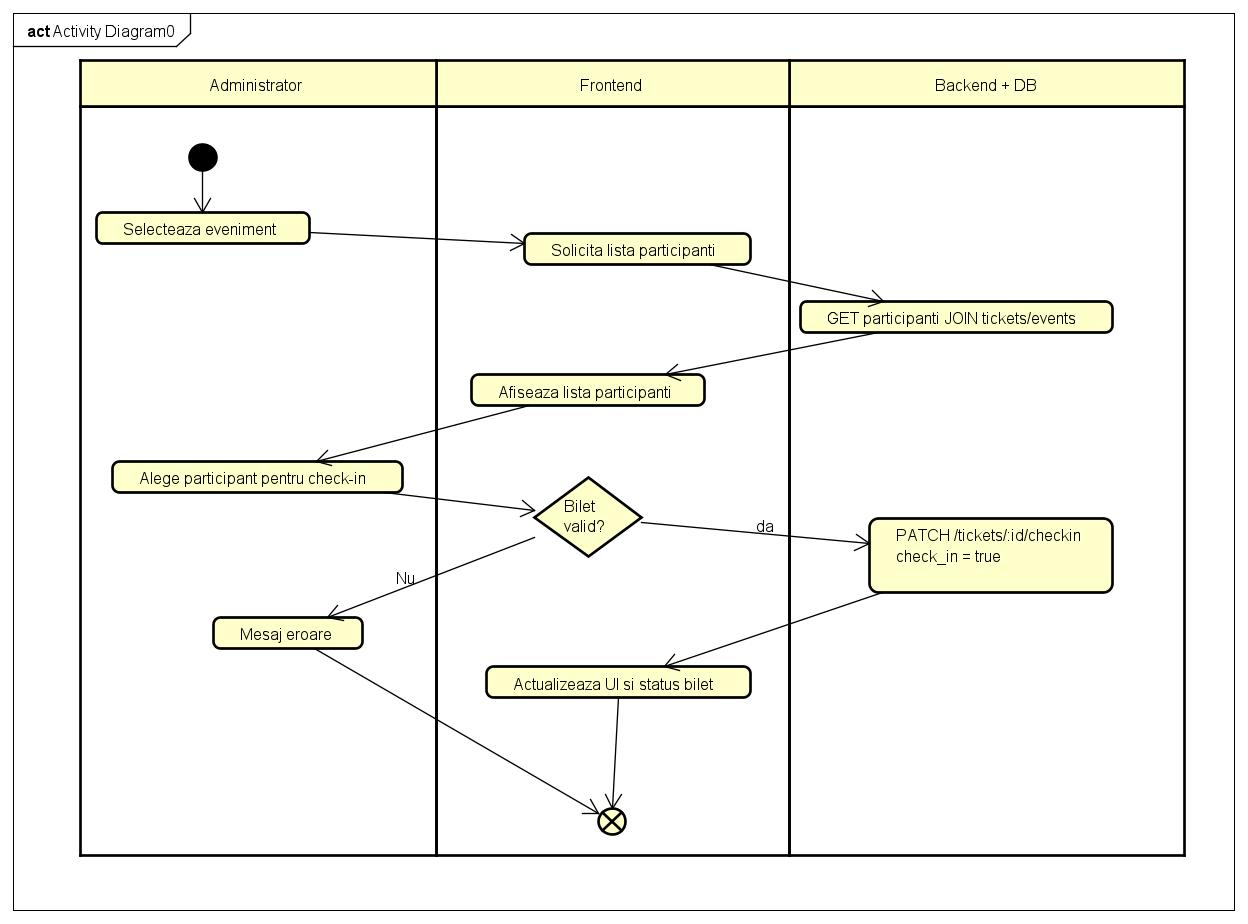
\includegraphics[width=1\textwidth]{Activity Diagram0.jpg}
	\caption{Diagrama de activitate - check-in}
	\label{fig:l2f1}
\end{figure}

\subsection{Proiectarea bazei de date}

Tabele principale: \texttt{users, events, tickets, password\_reset\_tokens, \linebreak registration\_verifications}

Rela\c tii: \texttt{events} 1:N \texttt{tickets; users} 1:N \texttt{tickets} (ON DELETE SET NULL); \texttt{users} 1:N token-uri reset; verific\u ari \^inregistrare temporare p\^an\u a la confirmare. 

\begin{figure}[htbp]
	\centering
	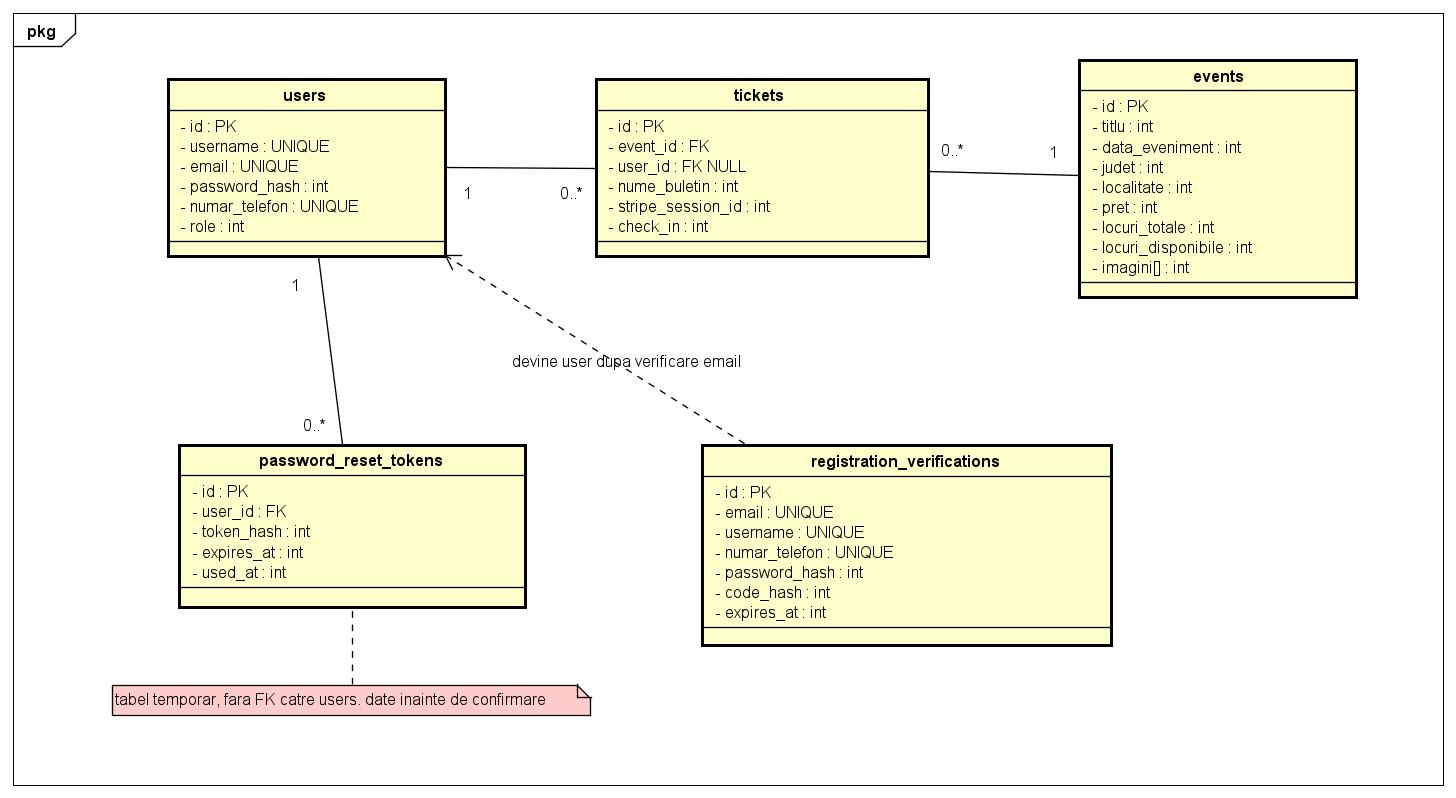
\includegraphics[width=1\textwidth]{Model de domeniu _ ERD ManFast.jpg}
	\caption{Diagrama entitate- rela\c tie}
	\label{fig:l2f1}
\end{figure}


\section{Proiectarea bazei de date}





Tabele principale: \texttt{user, events, tickets, password\_reset\_token, \linebreak registration\_verifi}

Rela\c tii: \texttt{events} 1:N \texttt{tickets; user} 1:N \texttt{tickets} (ON DELETE SET NULL) \texttt{user} 1:N token-uri reset \c si verific\u ari \^inregistrare temporare p\^an\u a la confirmare.




\section{Implementarea func\c tionalit\u a\c tilor cheie}
\subsection{Autentificarea \c si verificarea prin email}

Generarea codului \c si a hash-ului

\begin{lstlisting} 
	function genereazaCodVerificare() {
		return String(crypto.randomInt(100000, 1000000));
	}
	function hashCodVerificare(cod) {
		return crypto.createHash('sha256')
		.update(String(cod).trim()).digest('hex');
	}
\end{lstlisting}

La \texttt{POST /register/verify}, codul este comparat cu \texttt{code\_hash}, expirarea verificat\u a, apoi utilizatorul inserat \^in \texttt{users}. Login-ul genereaz\u a JWT: 

\begin{lstlisting}
	const token = jwt.sign(
	{ id: user.id, role: user.role },
	process.env.JWT_SECRET,
	{ expiresIn: '24h' }
	);
\end{lstlisting}

\subsection{Pl\u a\c ti prin Scripe}

Crearea sesiunii Checkout (extras):

\begin{lstlisting}
	const session = await stripe.checkout.sessions.create({
		payment_method_types: ['card'],
		line_items: [{ 
			price_data: {
				currency: 'ron',
				product_data: { name: `Bilet - ${event.titlu}` },
				unit_amount: Math.round(Number(event.pret) * 100),
			}, 
			quantity: cantitate 
		}],
		mode: 'payment',
		success_url: `${frontendUrl}/payment-success?session_id={CHECKOUT_SESSION_ID}`,
		metadata: { 
			event_id, 
			user_id, 
			nume_participanti: JSON.stringify(nume)
		}
	});
\end{lstlisting}

\texttt{confirm-payment} verific\u a \texttt{session.payment\_status} === '\texttt{paid}', insereaz\u a
c\^ate un r\^and \texttt{tickets} per nume \c si decrementeaz\u a \texttt{locuri\_disponibile} \^intr-o tranzac\c tie.

\subsection{Gestionare evenimente}

Crearea evenimentului folose\c ste Multer pentru imagini \c si validare jude\c t din lista fix\u a (42 jude\c te). La INSERT, \texttt{locuri\_disponibile = locuri totale}. Editarea permite ad\u augare incremental\u a de imagini. \c Stergerea elimin\u a evenimentul \c si biletele asociate (CASCADE)

\subsection{Frontend}

\texttt{AuthContext} stocheaz\u a \texttt{user} \c si \texttt{token} \^in \texttt{localStorage}. \texttt{apiFetch} \linebreak ata\c seaz\u aheader Authorization. Rute protejate: \texttt{/profile, /my-tickets, /admin} (AdminRoute).



\section{Securitate}

\begin{itemize}
	\item Parole: bcrypt cost 10; niciodat\u a \^in clar \^in DB.
	\item JWT: secret separat de Stripe; expirare 24h.
	\item Coduri email \c si token reset: SHA-256 \^in DB.
	\item Rate limit: max 3 coduri / 15 min (produc\c tie); cooldown 60s retrimitere.
	\item CORS: doar \texttt{FRONTEND\_URL}.
	\item Admin: ultimul admin protejat la \c stergere/revocare.
	\item \c Stergere cont: confirmare parol\u a obligatorie.
\end{itemize}

Implementarea respect\u a recomand\u arile OWASP [3] pentru autentificare \c si gestionarea sesiunilor \^in contextul unei aplica\c tii web educa\c tionale/prototip production-ready.

\section{Scenarii de utilizare pe tipuri de evenimente}

Aceast\u a sec\c tiune descrie modul \^in care acelea\c si func\c tionalit\u a\c ti ale platformei sunt valorificate \^in scenarii reprezentative. Scopul este de a demonstra flexibilitatea modelului simplu eveniment--bilet, f\u ar\u a a impune module separate per domeniu.

\subsection{Scenariul 1: Conferin\c t\u a universitar\u a}

Context: Facultatea organizeaz\u a o conferin\c t\u a \c stiin\c tific\u a cu 150 de locuri, taxa de participare 120 RON, desf\u a\c surare \^in Constan\c ta.

\hspace*{2ex} \textbf{Pa\c si organizator:}
\begin{enumerate}
	\item Administratorul creeaz\u a evenimentul: titlu, descriere (program, speakeri), dat\u a, jude\c t Constan\c ta, localitate, loca\c tie (sal\u a), pre\c t 120, locuri 150, durat\u a 8 ore, imagini (banner conferin\c t\u a).
	\item Public\u a link-ul c\u atre pagina principal\u a; participan\c tii filtreaz\u a dup\u a dat\u a sau jude\c t.
	\item Monitorizeaz\u a \texttt{locuri\_disponibile} \c si lista participan\c tilor.
	\item La intrare, efectueaz\u a check-in pe baza numelui de pe bilet.
\end{enumerate}

\textbf{Pa\c si organizator:} Pa\c si participant: \^inregistrare cont, verificare email, cump\u arare bilet nominal, prezentare la recep\c tie. Biletul din ``Biletele mele'' confirm\u a plata \c si identitatea.

\subsection{Scenariul 2 \^in care concertul este \^in aer liber}

\textbf{Context:} Asocia\c tie cultural\u a organizeaz\u a un concert local, 500 locrui, bilet 50 RON, galerie foto arti\c sti.

\textbf{Particularit\u a\c ti:} Galeria cu multiple imagini spore\c ste atractivitatea paginii de detalii. Filtrarea pe jude\c t ajut\u a publicul din zon\u a. V\^anzarea poate include mai multe bilete \^intr-o singur\u a tranzac\c tie Stripe (familie, grup de prieteni), fiecare nume completat corespunde unui bilet nominal.

\textbf{Limit\u ari actuale:} Nu exist\u a categorii de pre\c t (VIP, standard) sau hart\u a locurilor --- extensii posibile prin ad\u augarea unui c\^amp \texttt{tip\_bilet} \^in schema bazei de date.

\subsection{Scenariul 3: Meeting corporate / training}

\textbf{Context:} Firma de IT organizeaz\u a un workshop de o zi, 30 locuri, participare gratuit\u a sau cu pre\c t simbolic

Context: Club sportiv local, turneu cu taxa de \^inscriere, necesitate nume conform buletinului.
{Utilizare:} Chiar \c si la pre\c t mic, Stripe permite monetizare. Alternativ, organizatorul poate
seta pre\c t 1 RON pentru testare. Check-in-ul din admin ofer\u a lista de prezen\c t\u a pentru raport intern. Verificarea email la \^inregistrare reduce \^inscrierile fictive.

\subsection{Scenariul 4: Competi\c tie sportiv\u a amatorial\u a}

\textbf{Context:} Club sportiv local, turneu cu taxa de \^inscriere, necesitate nume conform buletinului.

\textbf{Utilizare:} C\^ampul \texttt{nume} buletin la cump\u arare capteaz\u a numele participantului. Check-in manual valideaz\u a prezen\c ta. Aceast\u a ni\c s\u a folose\c ste acelea\c si mecanisme ca conferin\c ta, f\u ar\u a tabele suplimentare pentru echipe sau clasamente. 

\subsection{Matricea func\c tionalit\u a\c tilor \c si scenarii}

\begin{table}[htbp]
	\centering
	\begin{tabular}{|l|c|c|c|c|}
		\hline
		\textbf{Func\c tionalitate} & \textbf{Conf.} & \textbf{Concert} & \textbf{Meeting} & \textbf{Sport} \\ \hline
		Filtrare jude\c t/dat\u a & Da & Da & Da & Da \\ \hline
		Galerie imagini & Da & Da & Op\c tional & Op\c tional \\ \hline
		Plat\u a Stripe RON & Da & Da & Da & Da \\ \hline
		Bilete multiple / tranzac\c tie & Da & Da & Rar & Da (echipe mici) \\ \hline
		Check-in admin & Da & Da & Da & Da \\ \hline
		Nume nominal (buletin) & Op\c tional & Op\c tional & Op\c tional & Da \\ \hline
	\end{tabular}
	\caption{Func\c tionalit\u a\c ti utilizate \^in scenarii}
	\label{tab:functionalitati_scenarii}
\end{table}

\subsection{Modelul unificat de date}

Decizia de a nu specializa tabelele per tip de eveniment (conferin\c t\u a vs. concert) simplific\u a mentenan\c ta \c si permite unui singur panou admin s\u a gestioneze toate formatele. C\^ampurile \texttt{titlu, descriere, data eveniment, judet, pret, locuri totale \linebreak si imagini} sunt suficient de generice; semantica (``taxa conferin\c t\u a'' vs. ``bilet concert'') este pur textual\u a, definit\u a de organizator.

Aceste scenarii pot fi reproducte \^in cadrul demonstra\c tiei aplica\c tiei \c si documentate prin capturi de ecran \^in capitolul 4.

\section{Fragmente suplimentare de implementare}
\subsection{Rate limiting la \^inregistrare}

Func\c tia depasesteLimitaCoduri limiteaz\u a abuzul de retrimitere cod email \^in produc\c tie:

\begin{lstlisting}
	function depasesteLimitaCoduri(row) {
		if (isDev) return null;
		
		const secundeDeLaUltimulCod =
		(Date.now() - new Date(row.last_code_sent_at).getTime()) / 1000;
		
		if (secundeDeLaUltimulCod < COOLDOWN_RETRIMITERE_SEC) {
			return { status: 429, error: 'Asteapta inainte de un cod nou.' };
		}
		
		if (inFereastraDe15Minute(row.last_code_sent_at)
		&& row.codes_sent >= MAX_CERERI_COD_15_MIN) {
			return { status: 429, error: 'Prea multe cereri de cod.' };
		}
		
		return null;
	}
\end{lstlisting}

\^In modul development (\texttt{NODE\_ENV} diferit de '\texttt{production}'), limitarea este dezactivat\u a pentru a facilita testarea repetat\u a a fluxului de \^inregistrare f\u ar\u a a a\c stepta cooldown-ul de 60 de secunde

\subsection{Middleware autentificare JWT}

Middleware-ul \texttt{authenticateToken} extrage token-ul din header \texttt{Authorization}: \texttt{Bearer}, verific\u a semn\u atura cu JWT\_SECRET \c si ata\c seaz\u a req.user pentru rutele protejate:

\begin{lstlisting}
	function authenticateToken(req, res, next) {
		const authHeader = req.headers['authorization'];
		const token = authHeader && authHeader.split(' ')[1];
		
		if (!token) return res.status(401).json({ error: 'Token lipsa' });
		
		jwt.verify(token, process.env.JWT_SECRET, (err, user) => {
			if (err) return res.status(403).json({ error: 'Token invalid' });
			req.user = user;
			next();
		});
	}
\end{lstlisting}

\texttt{requireAdmin} verific\u a suplimentar \texttt{req.user.role === 'admin'}, return\^and 403 pentru utilizatori obi\c snui\c ti. Aceast\u a separare permite reutilizarea autentific\u arii pe rute mixte (ex. /auth/me vs. /events POST).

\subsection{Validare evenimente la creare}

La \texttt{POST /events}, backend-ul valideaz\u a jude\c tul din lista fix\u a, pre\c tul pozitiv, locuri disponibile \c si proceseaz\u a upload-ul Multer:

\begin{lstlisting}
	const JUDETE_VALIDE = ['Alba', 'Arad', ..., 'Vaslui', 'Vrancea'];
	
	if (!JUDETE_VALIDE.includes(judet)) {
		return res.status(400).json({ error: 'Judet invalid' });
	}
	
	const locuriTotale = parseInt(locuri_totale, 10);
	
	if (isNaN(locuriTotale) || locuriTotale < 1) {
		return res.status(400).json({ error: 'Locuri invalide' });
	}
\end{lstlisting}

Imaginile sunt salvate \^in \texttt{uploads/events/} cu nume unic (timestamp + random), iar URL-urile relative sunt stocate \^in coloana \texttt{imagini} de tip \texttt{TEXT[]}.

\subsection{Componenta AdminRoute (frontend)}
Ruta \texttt{/admin} este protejat\u a pe client prin verificarea rouluiu din contex:

\begin{lstlisting}
	function AdminRoute({ children }) {
		const { user, loading } = useAuth();
		
		if (loading) return <CircularProgress />;
		
		if (!user || user.role !== 'admin') {
			return <Navigate to="/login" replace />;
		}
		
		return children;
	}
\end{lstlisting}

Protec\c tia pe client este complementar\u a, nu substitut pentru requireAdmin pe server --- orice apel API admin f\u ar\u a token valid este respins indiferent de manipularea rutei React. 

\subsection{Gestionare erori \c si feedback utilizator}

Frontend-ul centralizeaz\u a apelurile API \^in \texttt{apiFetch}, interpret\^and r\u aspunsurile JSON \c si afi\c seaz\u a mesaje Material UI (\texttt{Alert, Snackbar}). Codurile HTTP 400/401/403/429/500 sunt mapate la texte \^in rom\^an\u a \^in componentele de formular.

Backend-ul returneaz\u a structuri consistente \{\texttt{error: string} \} evit\^and expunerea stack trace \^in produc\c tie. Logging-ul pe consola ( \texttt{console.error}) assista debugging-ul \^in development.

Aceste fragmente ilustreaz\u a detalii de implementare care completeaz\u a diagramele \c si tabelele API, oferind cititorului o imagine concret\u a a codului surs\u a ManFast. 

\section{Modelul rela\c tional - detaliu tavele}
\subsection{Tabel user}

Stocheaz\u a conturile utilizatorilor. C\^ampuri: \texttt{id} (SERIAL PK), \texttt{username} (UNIQUE), \texttt{email} (UNIQUE), \texttt{password\_hash, numar\_telefon} (UNIQUE), \texttt{role} \linebreak (\texttt{user---admin}), \texttt{created\_at}. Rolul determin\u a accesul la  \texttt{/admin}.

Evenimentele publicate de administratori: \texttt{titlu, descriere, data \linebreak eveniment, judet, localitate, locatie} (string compus pentru afi\c sare), \texttt{pret, locuri \linebreak totale, locuri disponib imagini} (TEXT[]), \texttt{durata ore}. La creare, \texttt{locuri \linebreak disponibile = locuri totale}. Filtrarea pe home exclude evenimente expirate (\texttt{data + durata < NOW()}).

\subsection{Tabele auxiliare}

\texttt{registration\_verifications} --- stocare temporar\u a \^inregistr\u arilor p\^an\u a la cod email. 
\texttt{password\_reset\_tokens} --- token hash SHA-256, expirare 1h, used\_at la consum.

\section{API REST - referin\c t\u a}

Prefix: \texttt{/api}. Tabelul 3.3 listeaz\u a endpoint-urile de autentificare.

\begin{table}[htbp]
	\centering
	\begin{tabular}{|>{\ttfamily}p{5.5cm}|c|l|}
		\hline
		\textbf{Endpoint} & \textbf{Metod\u a} & \textbf{Descriere} \\ \hline
		/auth/register & POST & Trimite cod verificare email \\ \hline
		/auth/register/verify & POST & Confirm\u a cod, creeaz\u a cont \\ \hline
		/auth/register/resend & POST & Retrimite cod \\ \hline
		/auth/login & POST & Autentificare, returneaz\u a JWT \\ \hline
		/auth/me & GET & Utilizator curent (JWT) \\ \hline
		/auth/profile & PUT & Actualizare profil \\ \hline
		/auth/password & PUT & Schimbare parol\u a \\ \hline
		/auth/account & DELETE & \c Stergere cont (parol\u a) \\ \hline
		/auth/forgot-password & POST & Solicitare reset \\ \hline
		/auth/reset-password & POST & Parol\u a nou\u a cu token \\ \hline
		/auth/admin/create & POST & Promovare admin \\ \hline
		/auth/admin/revoke & POST & Revocare admin \\ \hline
	\end{tabular}
	\caption{Endpoint-uri autentificare}
	\label{tab:endpoints_auth}
\end{table}

\begin{table}[htbp]
	\centering
	\begin{tabular}{|>{\ttfamily}p{5cm}|c|l|}
		\hline
		\textbf{Endpoint} & \textbf{Metod\u a} & \textbf{Descriere} \\ \hline
		/events & GET & List\u a public\u a evenimente viitoare \\ \hline
		/events/:id & GET & Detalii eveniment \\ \hline
		/events & POST & Creare (admin) \\ \hline
		/events/:id & PUT & Editare (admin) \\ \hline
		/events/:id & DELETE & \c Stergere (admin) \\ \hline
		/events/admin/list & GET & List\u a admin \\ \hline
		/tickets/create-\newline checkout-session & POST & Sesiune Stripe \\ \hline
		/tickets/confirm-\newline payment & POST & Confirmare plat\u a \\ \hline
		/tickets/my-tickets & GET & Biletele utilizatorului \\ \hline
		/tickets/admin/\newline participants & GET & Participan\c ti (admin) \\ \hline
	\end{tabular}
	\caption{Endpoint-uri evenimente \c si bilete}
	\label{tab:endpoints_evenimente_bilete}
\end{table}

\section{Configurare \c si deployment}
\subsection{Variabile de mdiu backend}

\texttt{DB\_*, JWT\_SECRET, STRIPE\_SECRET\_KEY, FRONTEND\_URL, SMTP\_*,\linebreak MAIL\_FROM,
	ADMIN\_AUTHORIZATION\_PASSWORD}. Frontend: \texttt{VITE\_API\_URL}.

\subsection{Migr\u ari baz\u a de date}

Scripturi npm: \texttt{setup-db, migrate-judet-localitate, migrate-\linebreak password-reset, migrate-email-verification, migrate-\linebreak multi-tickets.} Schema complet\u a \^in \texttt{database/schema.sql.}

\subsection{Flux instalare}

\begin{enumerate}
	\item \textbf{PostgreSQL:} \texttt{CREATE DATABASE manfast}
	\item \texttt{cd backend \&\& npm install \&\& npm run setup-db}
	\item Rulare migr\u ari incrementale dac\u a proiect existent
	\item \texttt{npm run dev} backend; \texttt{cd frontend \&\& npm run dev}
	\item \textbf{Promovare admin:} \texttt{npm run promote-admin -- email@exemplu.com}
\end{enumerate}

\subsection{Componente frontend}

\subsubsection{Rute React Router}
\texttt{/}, \texttt{/login}, \texttt{/register}, \texttt{/forgot-password}, \texttt{/reset-password}, \texttt{/events/:id}, \texttt{/profile}, \texttt{/my-tickets}, \texttt{/payment-success}, \texttt{/admin} (\texttt{AdminRoute}).

\subsubsection{Context autentificare}
\texttt{AuthContext} expune \texttt{user}, \texttt{token}, \texttt{login}, \texttt{logout}, \texttt{updateUser}. \textbf{Token JWT \^in localStorage}. La \texttt{apiFetch}, header \texttt{Authorization: Bearer}.

\subsubsection{Tem\u a vizual\u a}
\texttt{darkTheme.js} --- palet\u a cyan pe fundal \^intunecat. Componente refolosibile: \texttt{AuthCard}, \texttt{PageContainer}, \texttt{EventListItem}, \texttt{StatusChip}.


\subsection{Confirmare plat\u a --- pseudocod}

\begin{lstlisting}[mathescape=true]
	BEGIN transaction
	existing = SELECT tickets WHERE stripe_session_id
	IF existing.count >= cantitate THEN COMMIT; RETURN dejaProcesat
	FOR nume IN numeDeInserat:
	INSERT INTO tickets (event_id, user_id, nume_buletin, ...)
	UPDATE events SET locuri_disponibile -= count
	COMMIT
\end{lstlisting}

\noindent Idemponteu\c ta: reapelarea \texttt{confirm-payment} cu acela\c si \texttt{session\_id} nu dubleaz\u a \linebreak biletele.


\subsection{Testare manual\u a}

Scenariu recomandat pentru demonstra\c tie:
\begin{enumerate}
	\item \^inregistrare + cod email;
	\item login;
	\item filtrare evenimente;
	\item cump\u arare bilet Stripe test \texttt{4242...};
	\item verificare ,,Biletele mele``;
	\item promovare admin;
	\item publicare eveniment;
	\item check-in;
	\item editare profil;
	\item \c stergere cont test.
\end{enumerate}

Aceste detalii completeaz\u a documenta\c tia tehnic\u a necesar\u a pentru \^in\c telegerea \c si reproductibilitatea solu\c tiei ManFast. % OBLIGATORIU
\chapter{Prezentarea aplica\c tiei}

Aplica\c tia ManFast ruleaz\u a \^in browser la \texttt{http://localhost:5173} (frontend) \c si comunic\u a cu API-ul Express la portul 5000. \^In acest capitol sunt ilustrate interfe\c tele principale.

\section{Utilizarea aplica\c tiei — perspectiva \linebreak utilizatorului}

\subsection{Pagina principal\u a}

Pagina principal\u a afi\c seaz\u a evenimentele viitoare sub form\u a de list\u a orizontal\u a. Componenta \texttt{EventSearchFilters} permite filtrarea dup\u a nume, jude\c t (select din 42 jude\c te) \c si dat\u a. Evenimentele expirate (data + durata) nu apar \^in list\u a.

Utilizatorul neautentificat poate naviga \c si filtra evenimente. Pentru cump\u arare bilet este necesar\u a autentificarea. Designul folose\c ste carduri \texttt{EventListItem} cu titlu, loca\c tie, pre\c t \c si locuri disponibile. Navbar-ul con\c tine link-uri c\u atre ,,Evenimente``, ,,Biletele mele`` \c si ,,Profil`` (vizibile doar autentificat), plus buton ,,Panou Admin`` pentru rol admin.

Filtrarea pe jude\c t utilizeaz\u a lista complet\u a jude\c telor din \texttt{constants/judete.js}, aliniat\u a la organizarea administrativ\u a din Rom\^ania. Filtrul pe dat\u a permite restr\^angerea rezultatelor la o zi specific\u a, util \^in planificarea particip\u arii la competi\c tii.

\begin{figure}[htbp]
	\centering
	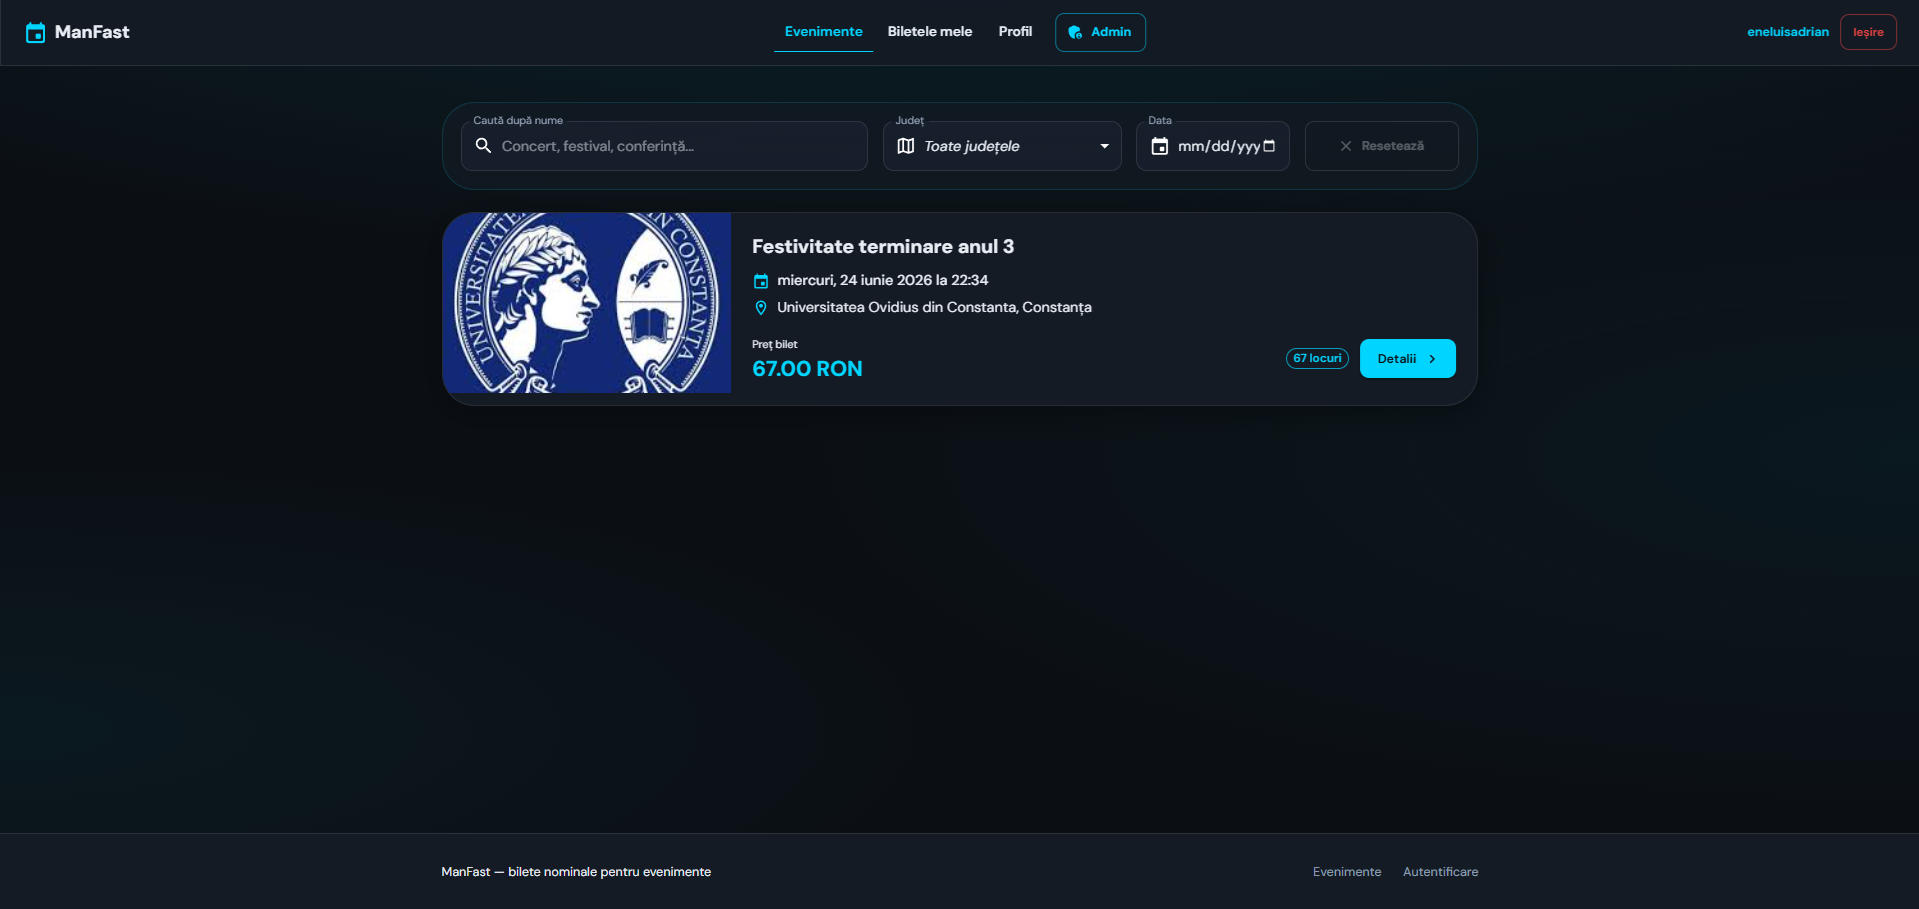
\includegraphics[width=1\textwidth]{paginaprincipala.png}
	\caption{Pagina principal\u a — list\u a evenimente \c si filtre}
	\label{fig:l2f1}
\end{figure}



\subsection{Detalii eveniment}

Pagina \texttt{/events/:id} prezint\u a titlul, galeria de imagini, descrierea, data, jude\c tul, localitatea, loca\c tia, pre\c tul \c si locurile disponibile. Utilizatorul autentificat poate ad\u auga unul sau mai multe c\^ampuri ,,Nume participant`` \c si ini\c tia plata Stripe.

Galeria de imagini suport\u a mai multe fi\c siere \^inc\u arcate de admin (max 8, 5MB/fi\c sier). Layout-ul este responsive: pe desktop, detaliile \c si formularul de cump\u arare pot ap\u area \^in coloane; pe mobil, stiv\u a vertical\u a. Validarea frontend verific\u a c\u a toate numele sunt completate \^inainte de apelul API. La succes, utilizatorul este redirectat c\u atre Stripe Checkout hosted page — datele cardului nu tranziteaz\u a serverul ManFast.



\begin{figure}[htbp]
	\centering
	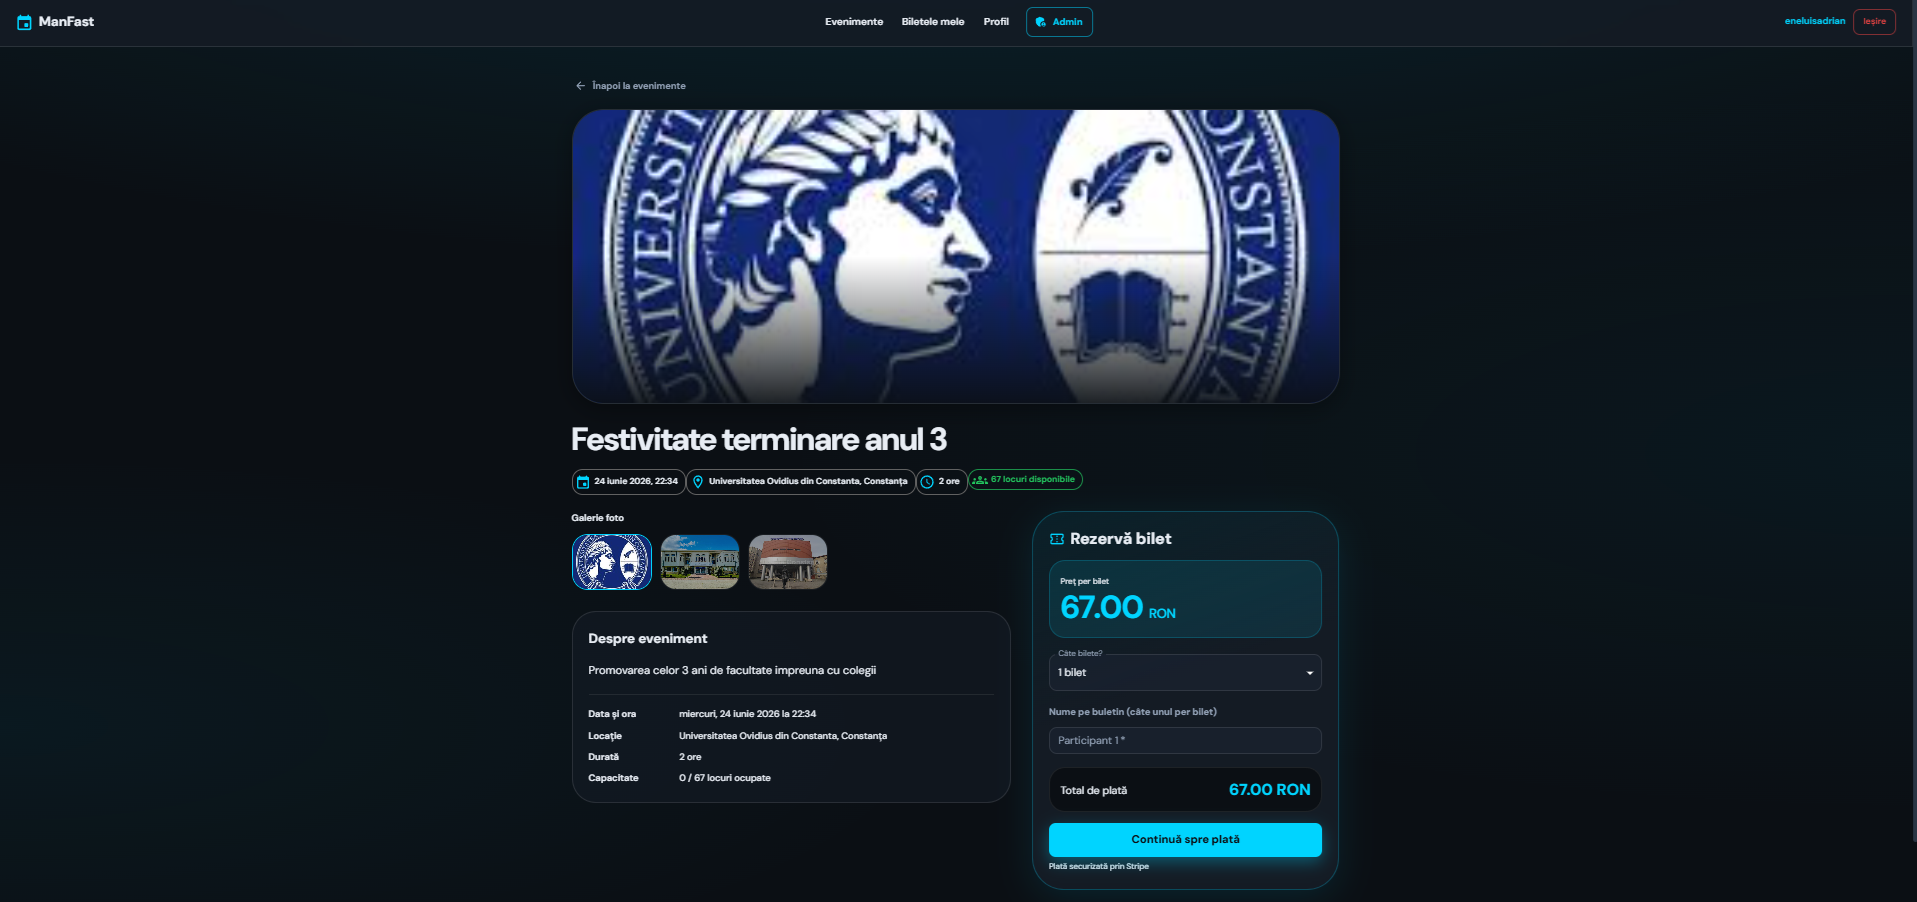
\includegraphics[width=1\textwidth]{Pagina_detalii_eveniment_si_formular_bilete.png}
	\caption{Pagina detalii eveniment \c si formular bilete}
	\label{fig:l2f1}
\end{figure}

\subsection{\^Inregistrare cont — pasul 1}

Formularul de \^inregistrare colecteaz\u a username, email, telefon, parol\u a. La submit se apeleaz\u a \texttt{POST /api/auth/register} \c si se trece la ecranul de verificare.

\begin{figure}[htbp]
	\centering
	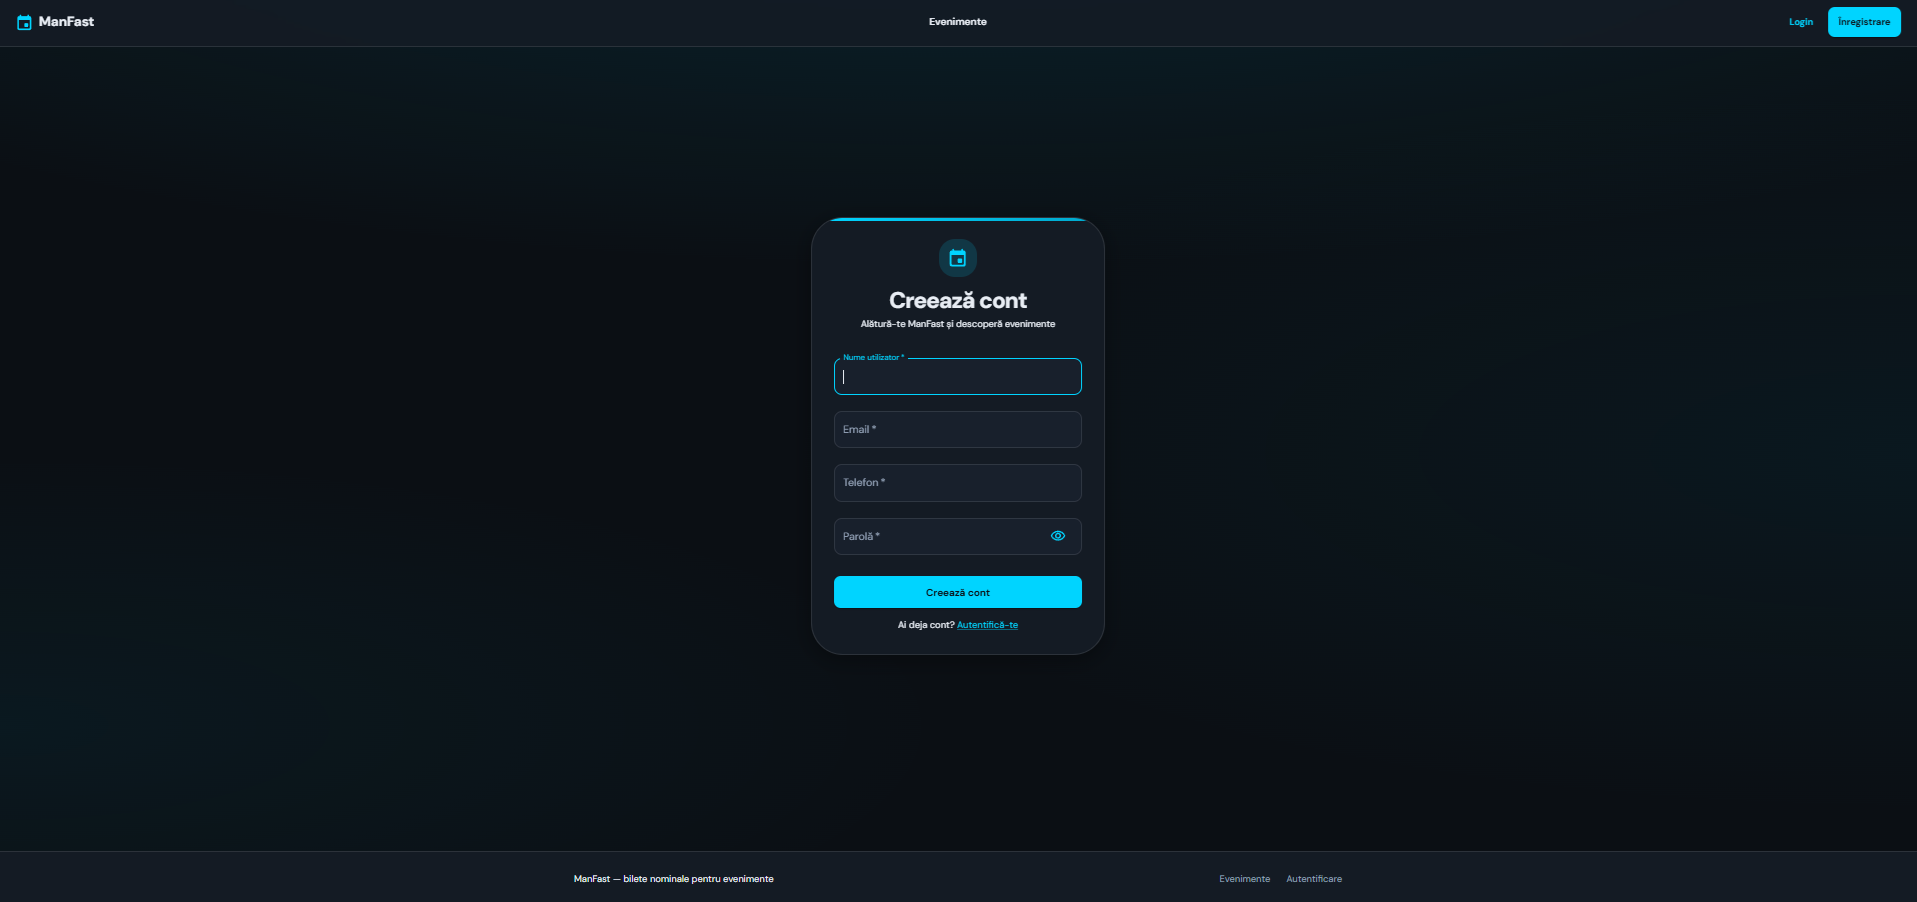
\includegraphics[width=1\textwidth]{Formular_inregistrare.png}
	\caption{Formular \^inregistrare}
	\label{fig:l2f1}
\end{figure}

\subsection{Verificare email — pasul 2}

Utilizatorul introduce codul de 6 cifre primit pe email. Op\c tiuni: retrimite cod, \^inapoi la formular.

\begin{figure}[htbp]
	\centering
	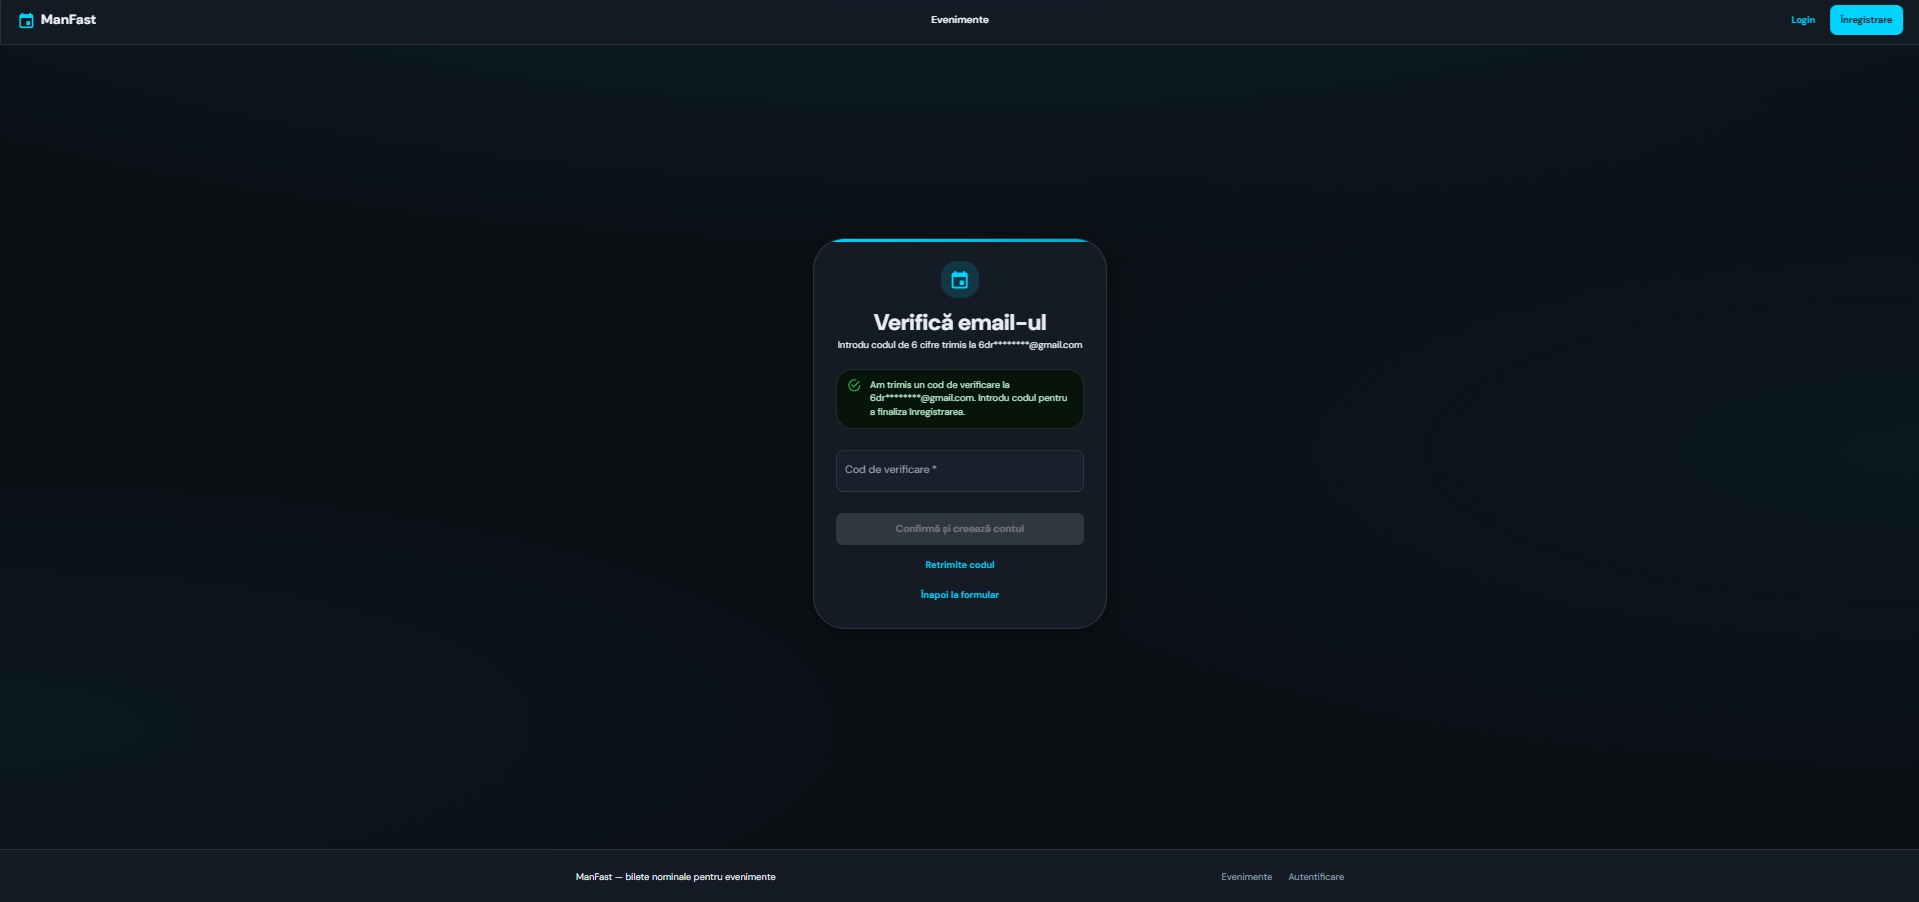
\includegraphics[width=1\textwidth]{Verificare email cu_cod.png}
	\caption{Verificare email cu cod}
	\label{fig:l2f1}
\end{figure}

\subsection{Autentificare}

Pagina \texttt{/login} permite autentificarea. Link-uri c\u atre ,,Am uitat parola`` \c si ,,\^Inregistreaz\u a-te`` (transfer email/parol\u a prin state).

\begin{figure}[htbp]
	\centering
	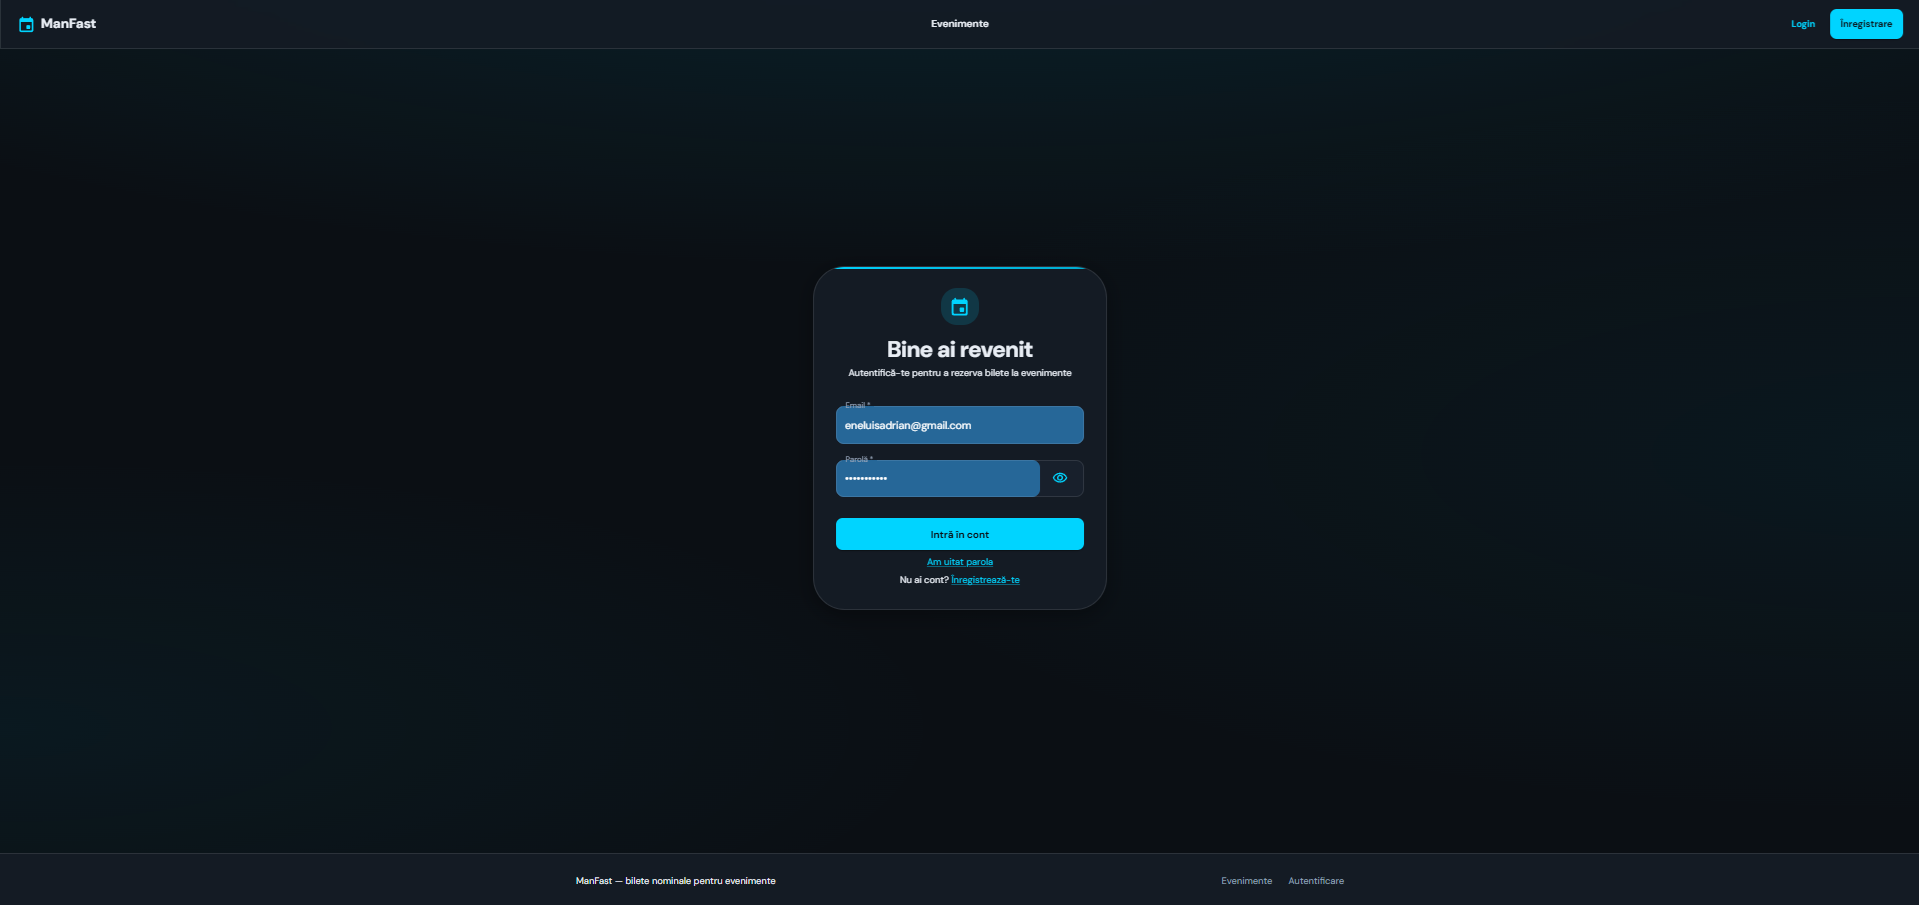
\includegraphics[width=1\textwidth]{Pagina login.png}
	\caption{Pagina login}
	\label{fig:l2f1}
\end{figure}

\subsection{Confirmare plat\u a}

Dup\u a Stripe Checkout, utilizatorul revine la \texttt{/payment-success?session\_id=...}. Frontend confirm\u a plata \c si redirec\c tioneaz\u a spre bilete.

\begin{figure}[htbp]
	\centering
	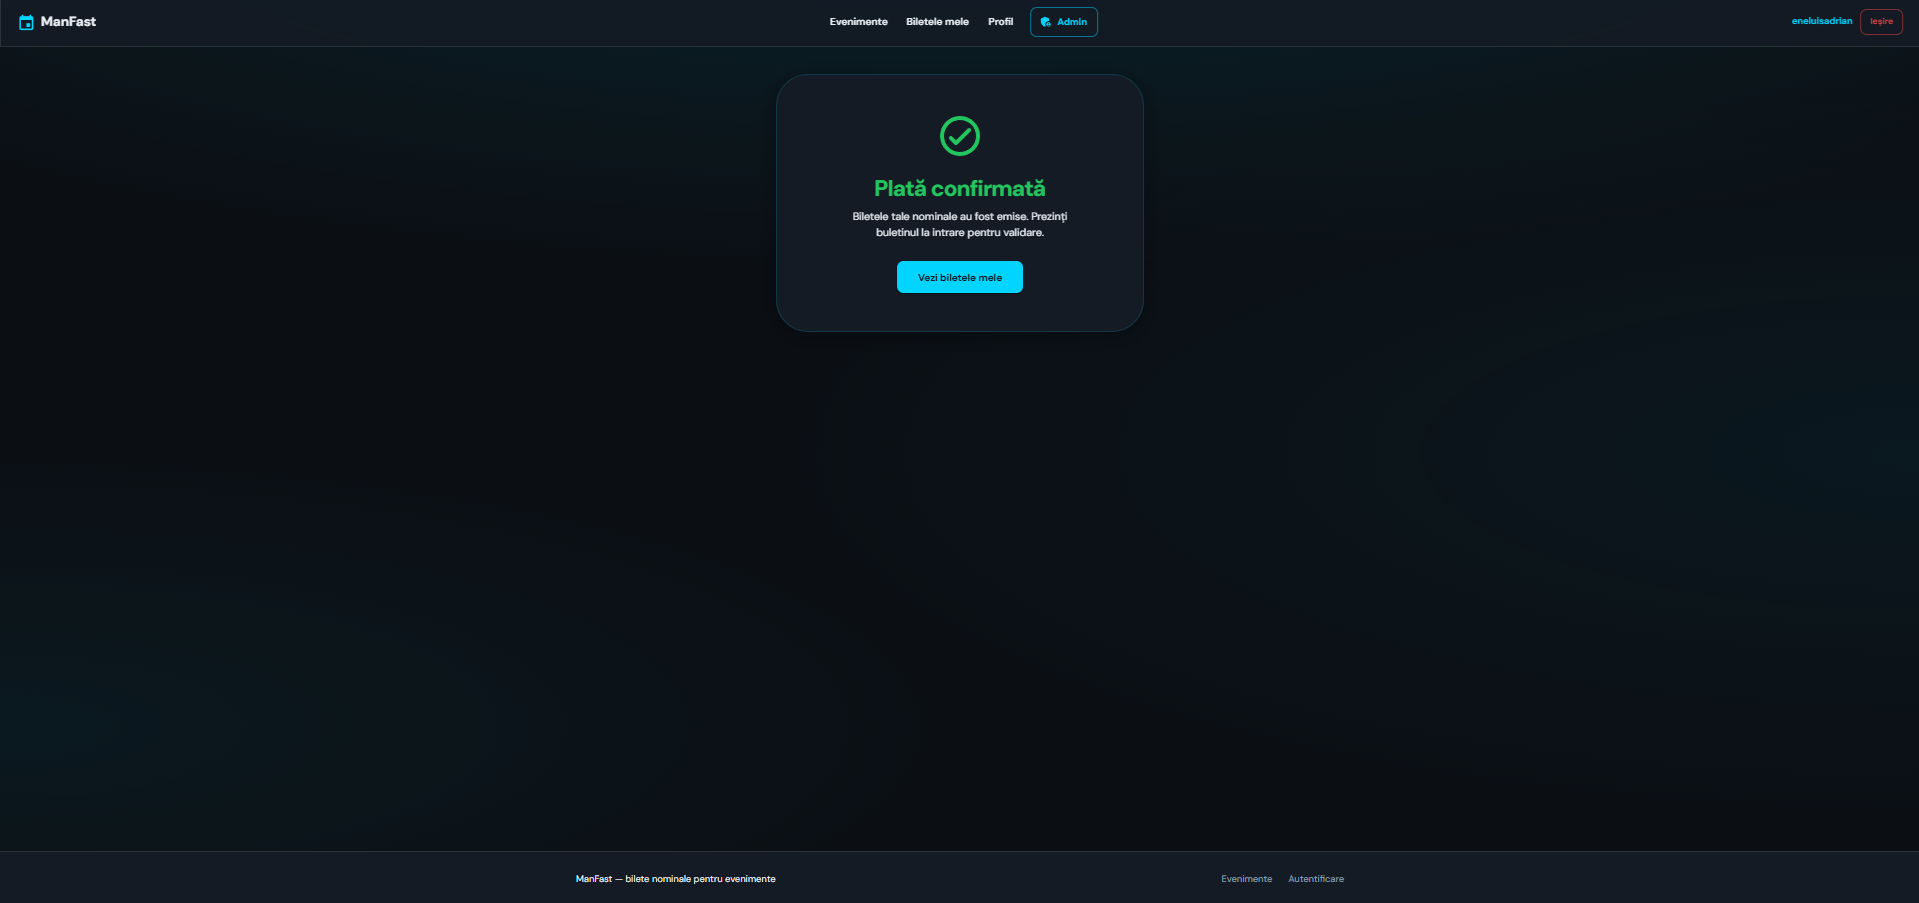
\includegraphics[width=1\textwidth]{Pagina succes plat ˘ a.png}
	\caption{Pagina succes plat\u a}
	\label{fig:l2f1}
\end{figure}

\subsection{Biletele mele}

\texttt{/my-tickets} grupeaz\u a biletele \^in ,,viitoare`` \c si ,,trecute``. Fiecare card arat\u a evenimentul, numele de pe bilet, status (Pl\u atit / Check-in / Expirat).

\begin{figure}[htbp]
	\centering
	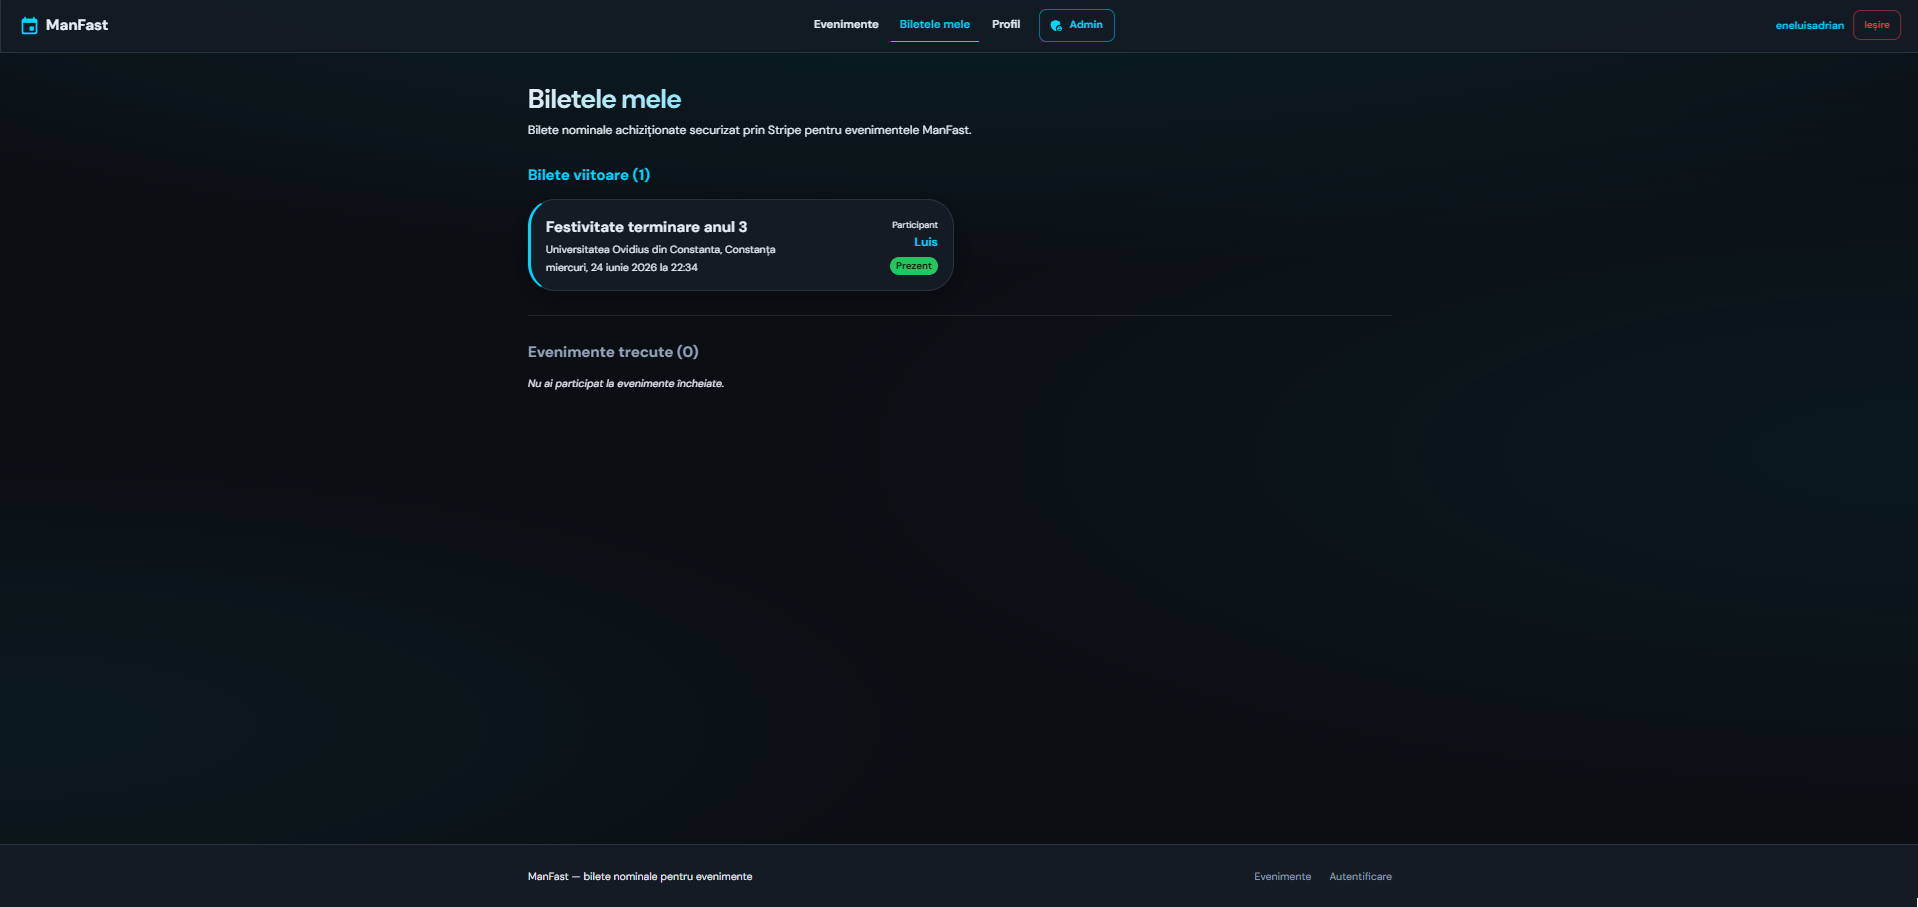
\includegraphics[width=1\textwidth]{Biletele mele.png}
	\caption{Biletele mele}
	\label{fig:l2f1}
\end{figure}

\subsection{Profil utilizator}

\texttt{/profile}: mod vizualizare \c si mod editare; schimbare parol\u a; zon\u a ro\c sie \c stergere cont.

\begin{figure}[htbp]
	\centering
	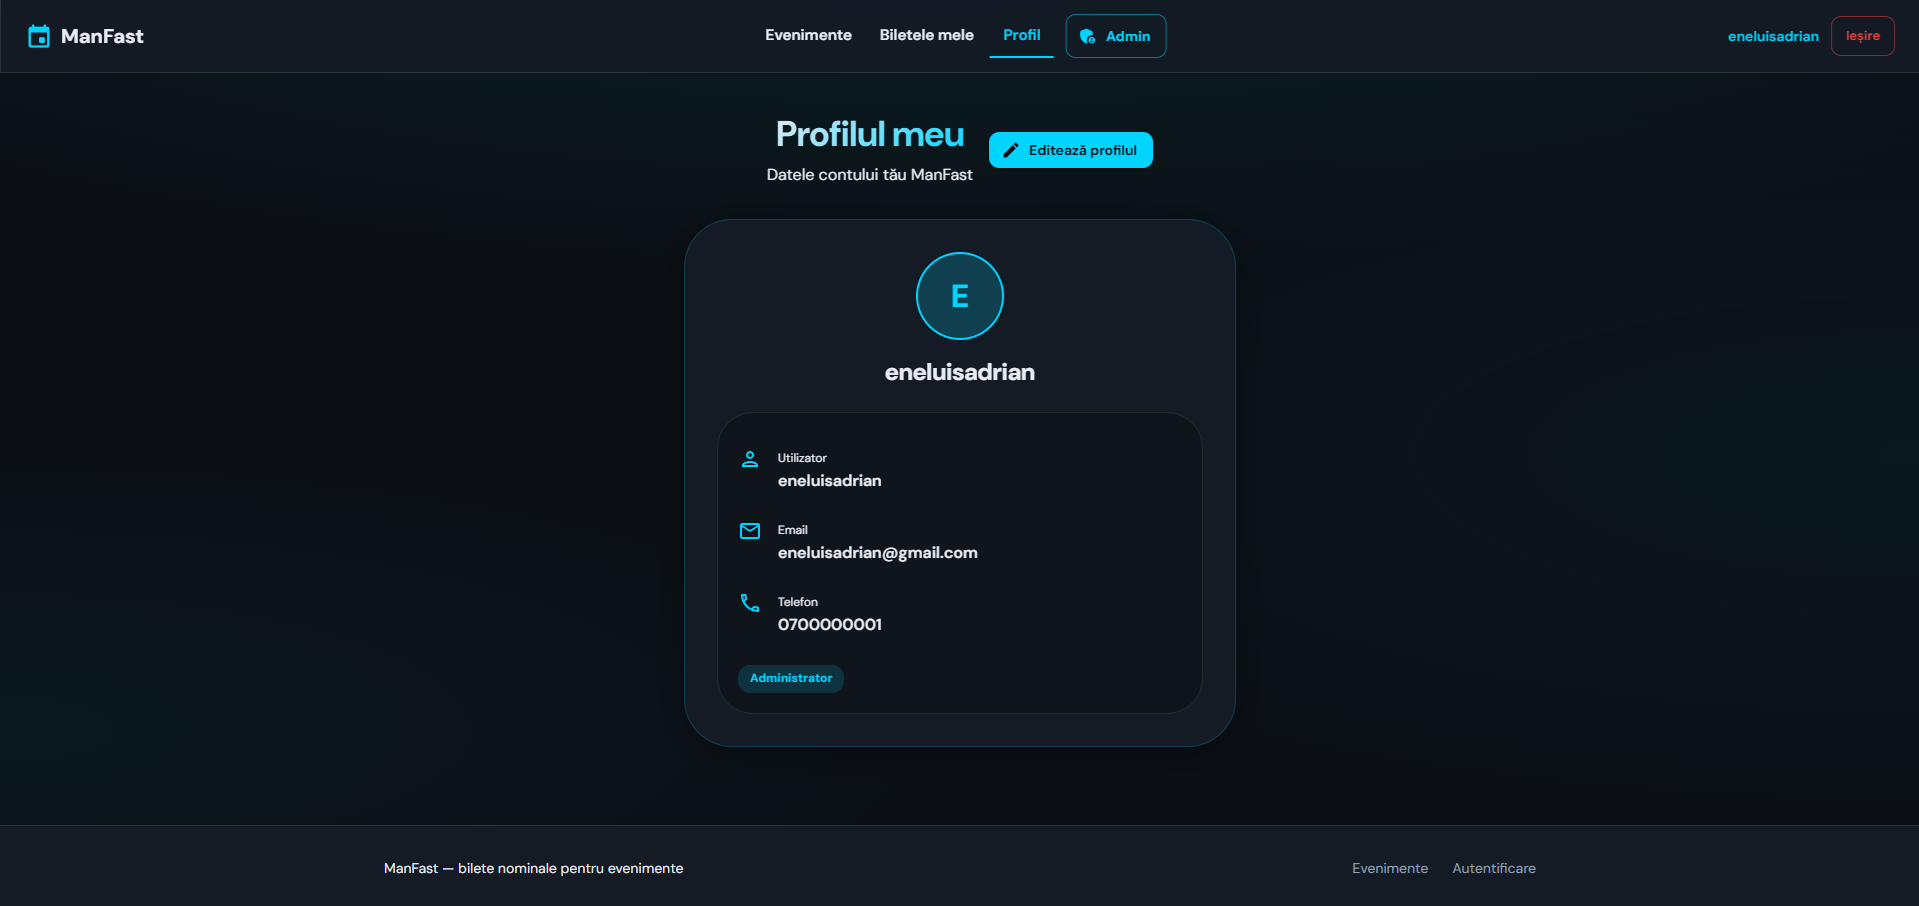
\includegraphics[width=1\textwidth]{Profil utilizator.png}
	\caption{Profil utilizator}
	\label{fig:l2f1}
\end{figure}

\subsection{Resetare parol\u a — pasul 1 (op\c tional)}

Formularul ,,Am uitat parola`` accept\u a email sau telefon; backend-ul trimite link de reset pe email (mesaj generic pentru confiden\c tialitate).

\begin{figure}[htbp]
	\centering
	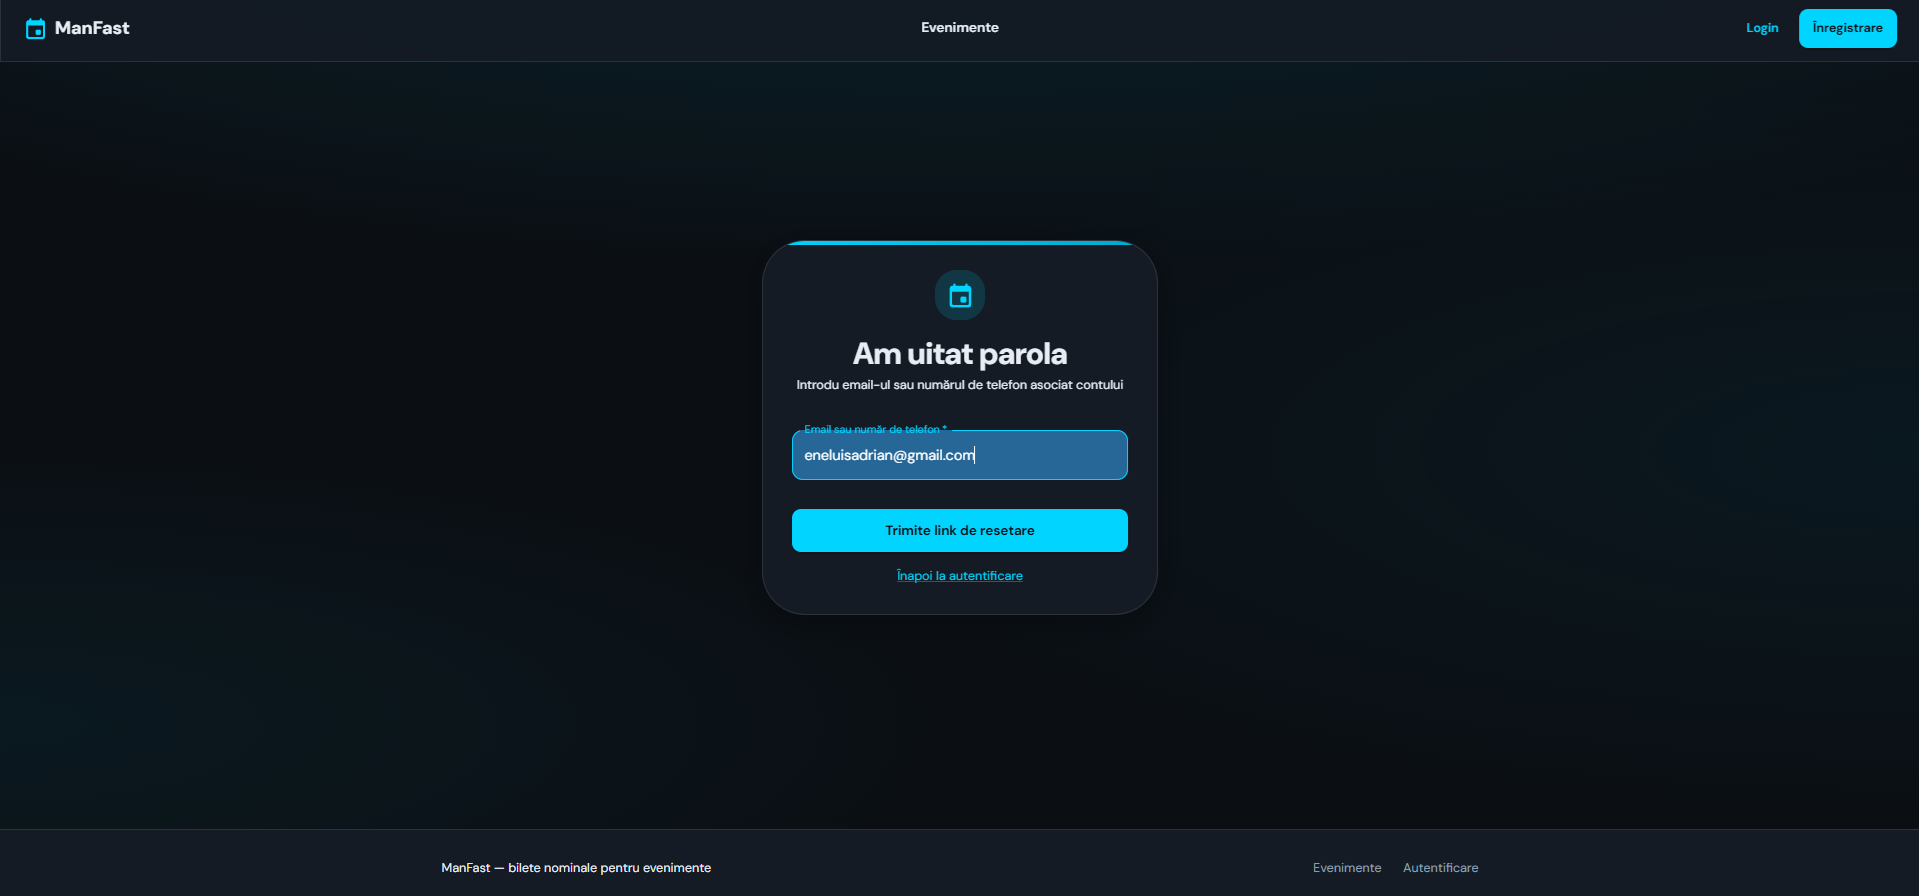
\includegraphics[width=1\textwidth]{Pagina Am uitat parola (opt¸ional).png}
	\caption{Pagina Am uitat parola (op\c tional)}
	\label{fig:l2f1}
\end{figure}

\subsection{Resetare parol\u a — pasul 2 (op\c tional)}

Dup\u a solicitarea reset\u arii, utilizatorul acceseaz\u a link-ul din email (\texttt{/reset-password-\linebreak token=...}) \c si seteaz\u a parola nou\u a. Token-ul este validat server-side (hash SHA-256, expirare 1h).

\begin{figure}[htbp]
	\centering
	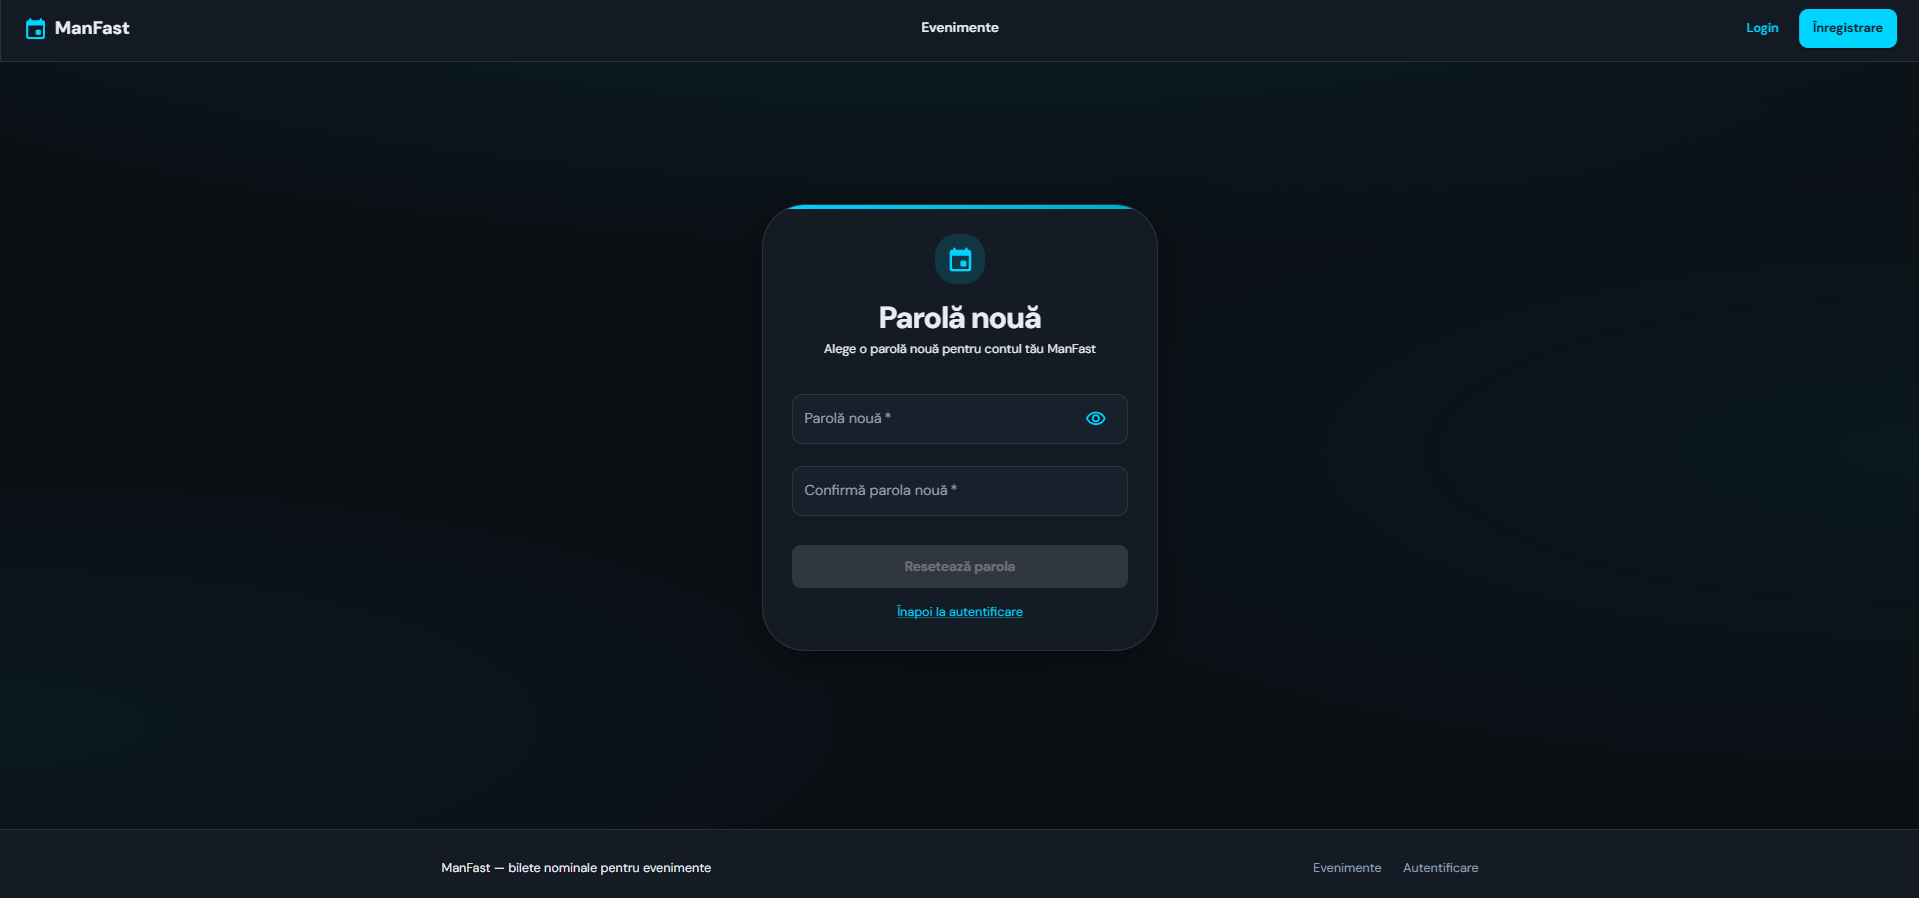
\includegraphics[width=1\textwidth]{Formular parola nou ˘ a (reset).png}
	\caption{Formular parola nou\u a (reset)}
	\label{fig:l2f1}
\end{figure}


\section{Experien\c ta utilizatorului \c si design responsive}

\subsection{Parcursul utilizatorului (user journey)}

Fluxul complet al unui participant nou poate fi rezumat astfel: descoperire eveniment pe Home $\rightarrow$ consultare detalii $\rightarrow$ redirect la Login/Register dac\u a nu este autentificat $\rightarrow$ \linebreak \^inregistrare cu verificare email $\rightarrow$ revenire la eveniment $\rightarrow$ completare nume participan\c ti $\rightarrow$ plat\u a Stripe $\rightarrow$ confirmare $\rightarrow$ vizualizare bilet \^in Biletele mele $\rightarrow$ prezentare la check-in (validat de admin)

Fiecare pas este marcat de feedback vizual: st\u ari de \^inc\u arcare (\texttt{CircularProgress}), mesaje de eroare contextualizate, redirect automat dup\u a ac\c tiuni reu\c site. Transferul email/\linebreak parol\u a de la Login la Register (via \texttt{location.state}) reduce fric\c tiunea pentru utilizatorii care \^incep de pe pagina gre\c sit\u a.

\subsection{Adaptare mobil \c si accesibilitate}

Material UI 9 ofer\u a componente responsive (\texttt{Grid}, \texttt{Stack}, \texttt{useMediaQuery}). Navbar-ul comut\u a la meniul hamburger pe ecrane \^inguste; filtrele pe Home se stiveaz\u a vertical. Formularele de autentificare sunt centrate \^in \texttt{AuthCard} cu l\u a\c time maxim\u a, u\c sor de utilizat pe telefon.

Au fost remediate probleme de accesibilitate: focus corect dup\u a \^inchiderea meniului mobil (evitare \texttt{aria-hidden} pe elemente focusabile), utilizarea etichetelor \texttt{label} pe c\^ampuri, contrast ridicat \^in tema dark (cyan pe fundal \^intunecat).

\subsection{Mesaje de eroare \c si st\u ari goale}

Listele goale (f\u ar\u a evenimente, f\u ar\u a bilete) afi\c seaz\u a text explicativ \c si sugestii (ex. ,,Modific\u a filtrele`` sau ,,Cump\u ar\u a primul bilet``). Erorile API (429 rate limit, 401 sesiune expirat\u a) sunt traduse \^in mesaje inteligibile, f\u ar\u a detalii tehnice expuse utilizatorului final.

\section{Utilizarea aplica\c tiei — perspectiva administratorului}

Administratorul acceseaz\u a \texttt{/admin} dup\u a autentificare cu rol \texttt{admin}. Componenta \linebreak \texttt{AdminRoute} verific\u a token JWT \c si rol; utilizatorii obi\c snui\c ti sunt redirec\c tiona\c ti.

Panoul centralizeaz\u a gestionarea evenimentelor \c si a participan\c tilor. Administratorul poate crea evenimente noi, edita pe cele existente (inclusiv ad\u augare imagini incremental), \c sterge evenimente (cu confirmare dialog) \c si vizualiza participan\c ti cu status check-in. Gestionarea administratorilor se face \^intr-un dialog separat, protejat de parol\u a de autorizare configurat\u a \^in \texttt{.env}.

\subsection{Panou admin — dashboard}

List\u a evenimente cu ac\c tiuni editare/\c stergere; tab participan\c ti; check-in.

\begin{figure}[htbp]
	\centering
	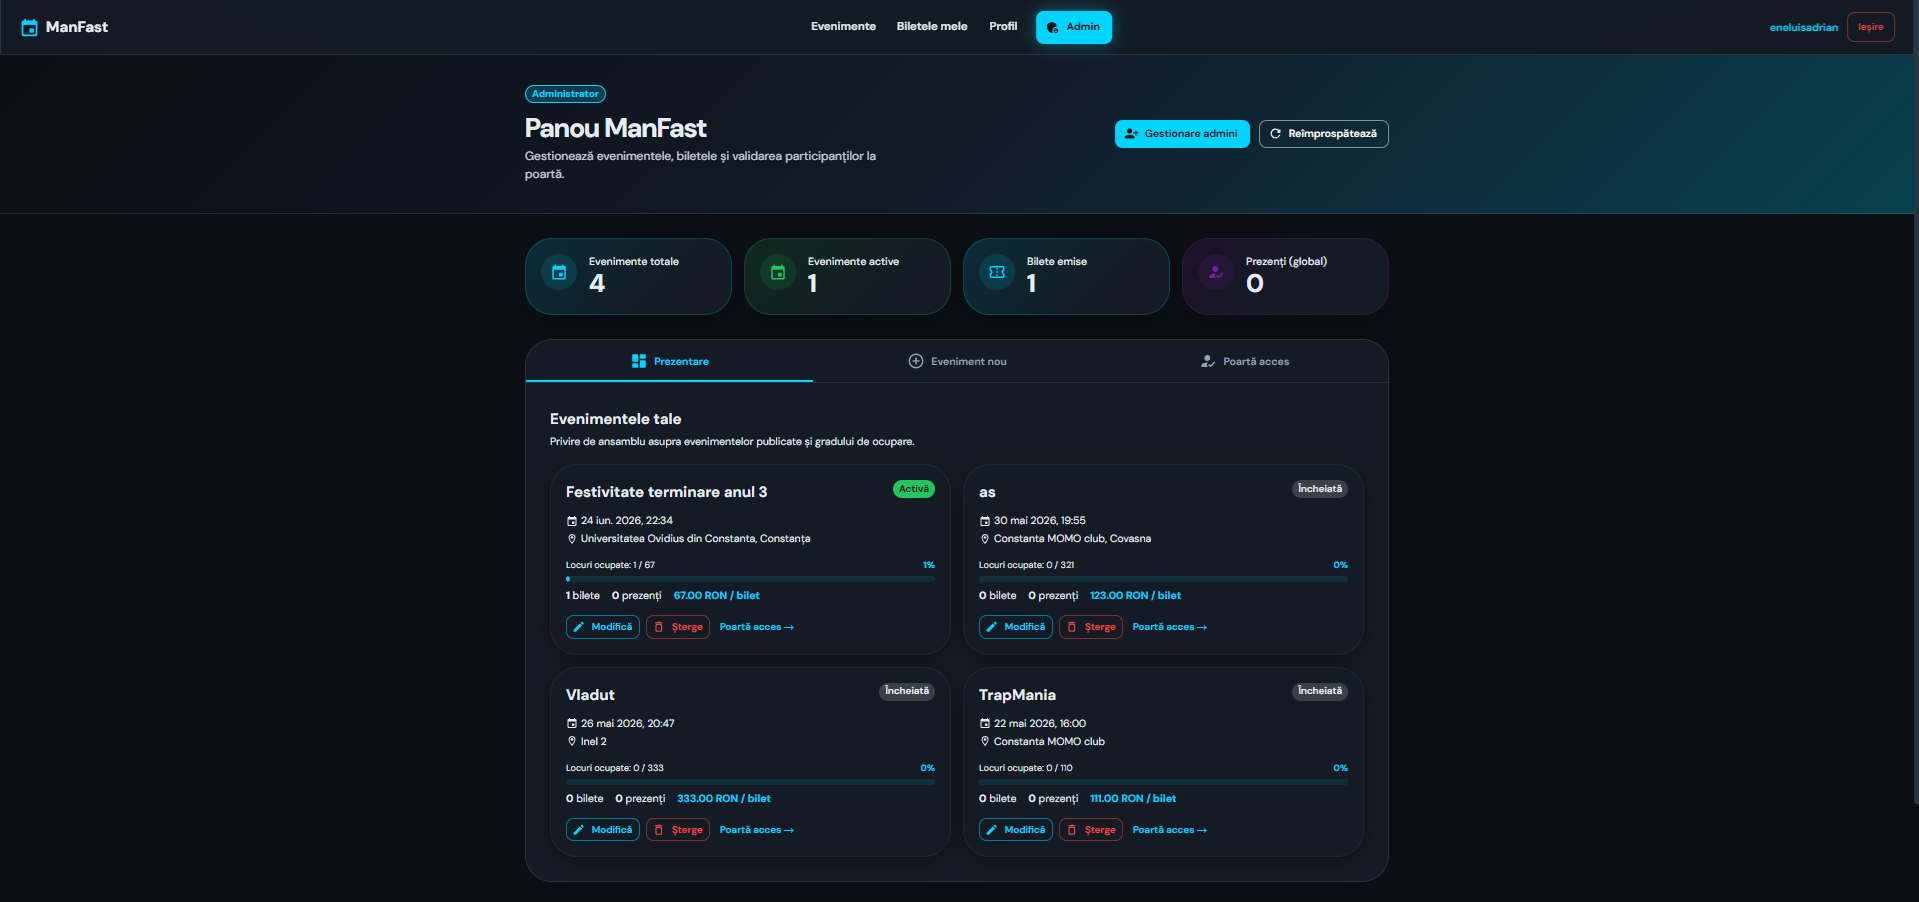
\includegraphics[width=1\textwidth]{Panou admin — dashboard.png}
	\caption{Panou admin — dashboard}
	\label{fig:l2f1}
\end{figure}

\subsection{Creare / editare eveniment}

Dialog cu c\^ampuri: titlu, descriere, dat\u a, jude\c t, localitate, pre\c t, locuri, durat\u a, upload imagini.

\begin{figure}[htbp]
	\centering
	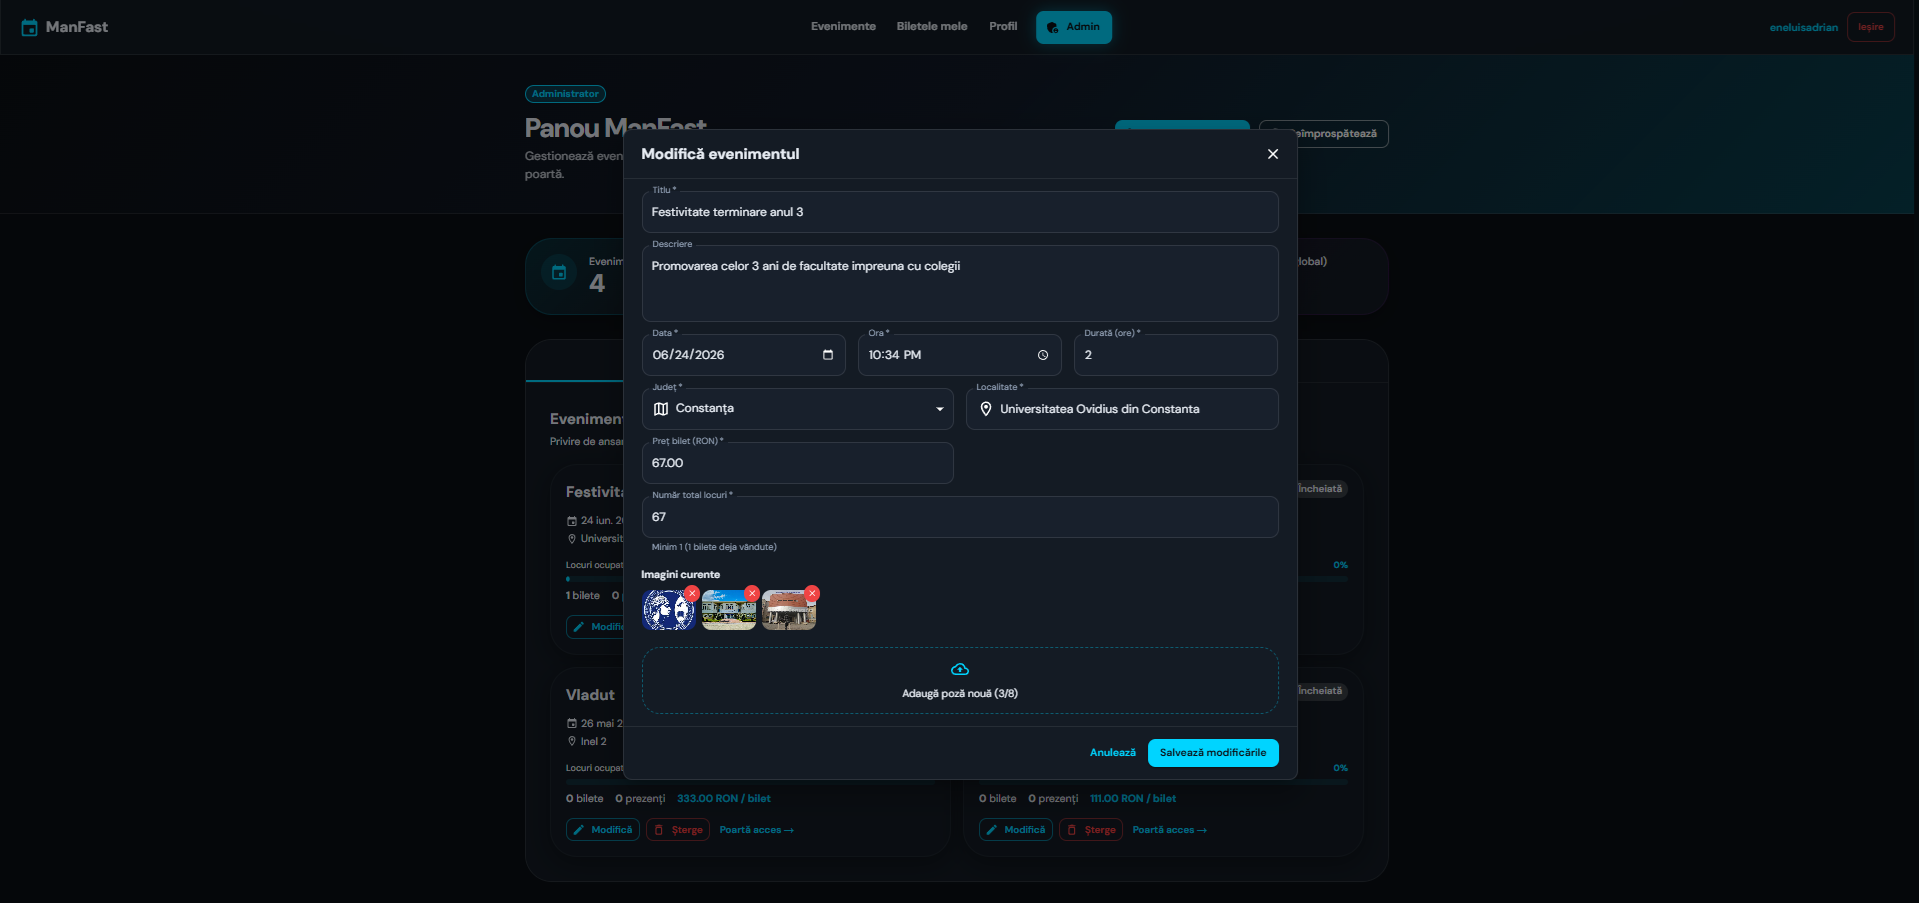
\includegraphics[width=1\textwidth]{Dialog editare eveniment.png}
	\caption{Dialog editare eveniment}
	\label{fig:l2f1}
\end{figure}

\subsection{Check-in participant}

Marcarea unui participant ca prezent (buton check-in sau toggle)

\begin{figure}[htbp]
	\centering
	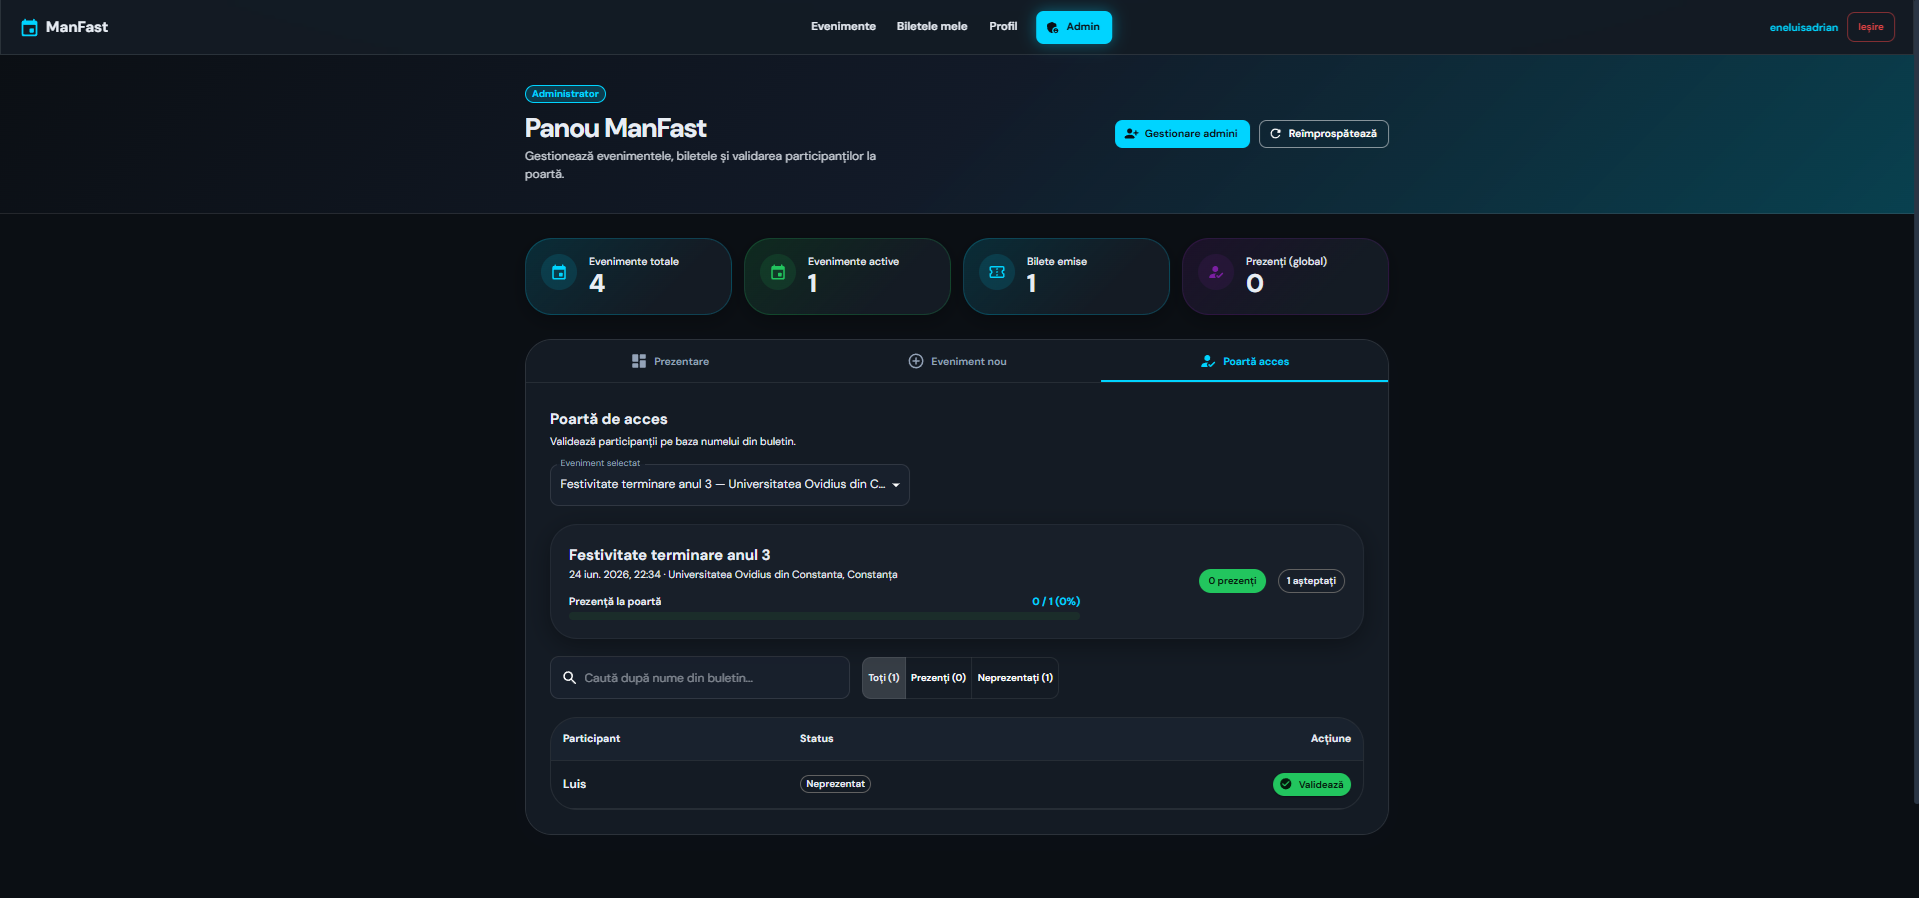
\includegraphics[width=1\textwidth]{Check-in participant.png}
	\caption{Check-in participant}
	\label{fig:l2f1}
\end{figure}

\begin{figure}[htbp]
	\centering
	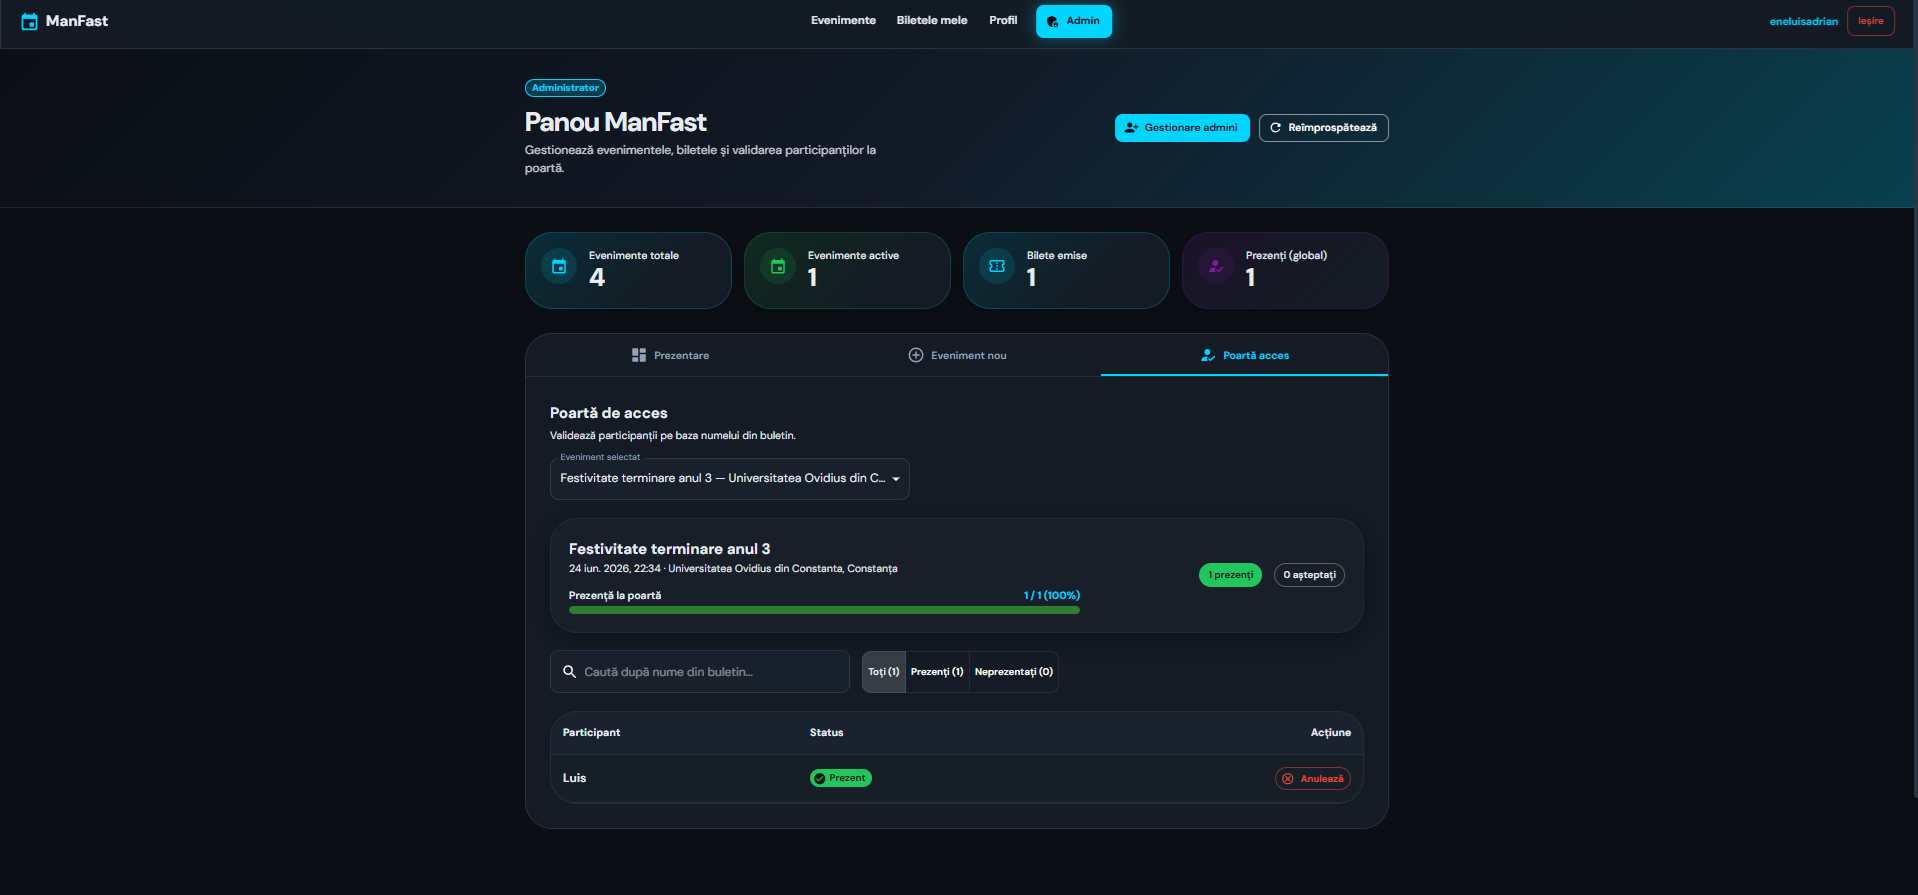
\includegraphics[width=1\textwidth]{Check-in participant2.png}
	\caption{Check-in participant validat}
	\label{fig:l2f1}
\end{figure}

\subsection{Gestionare administratori}

Dialog promovare sau revocare admin cu parol\u a autorizare.

\begin{figure}[htbp]
	\centering
	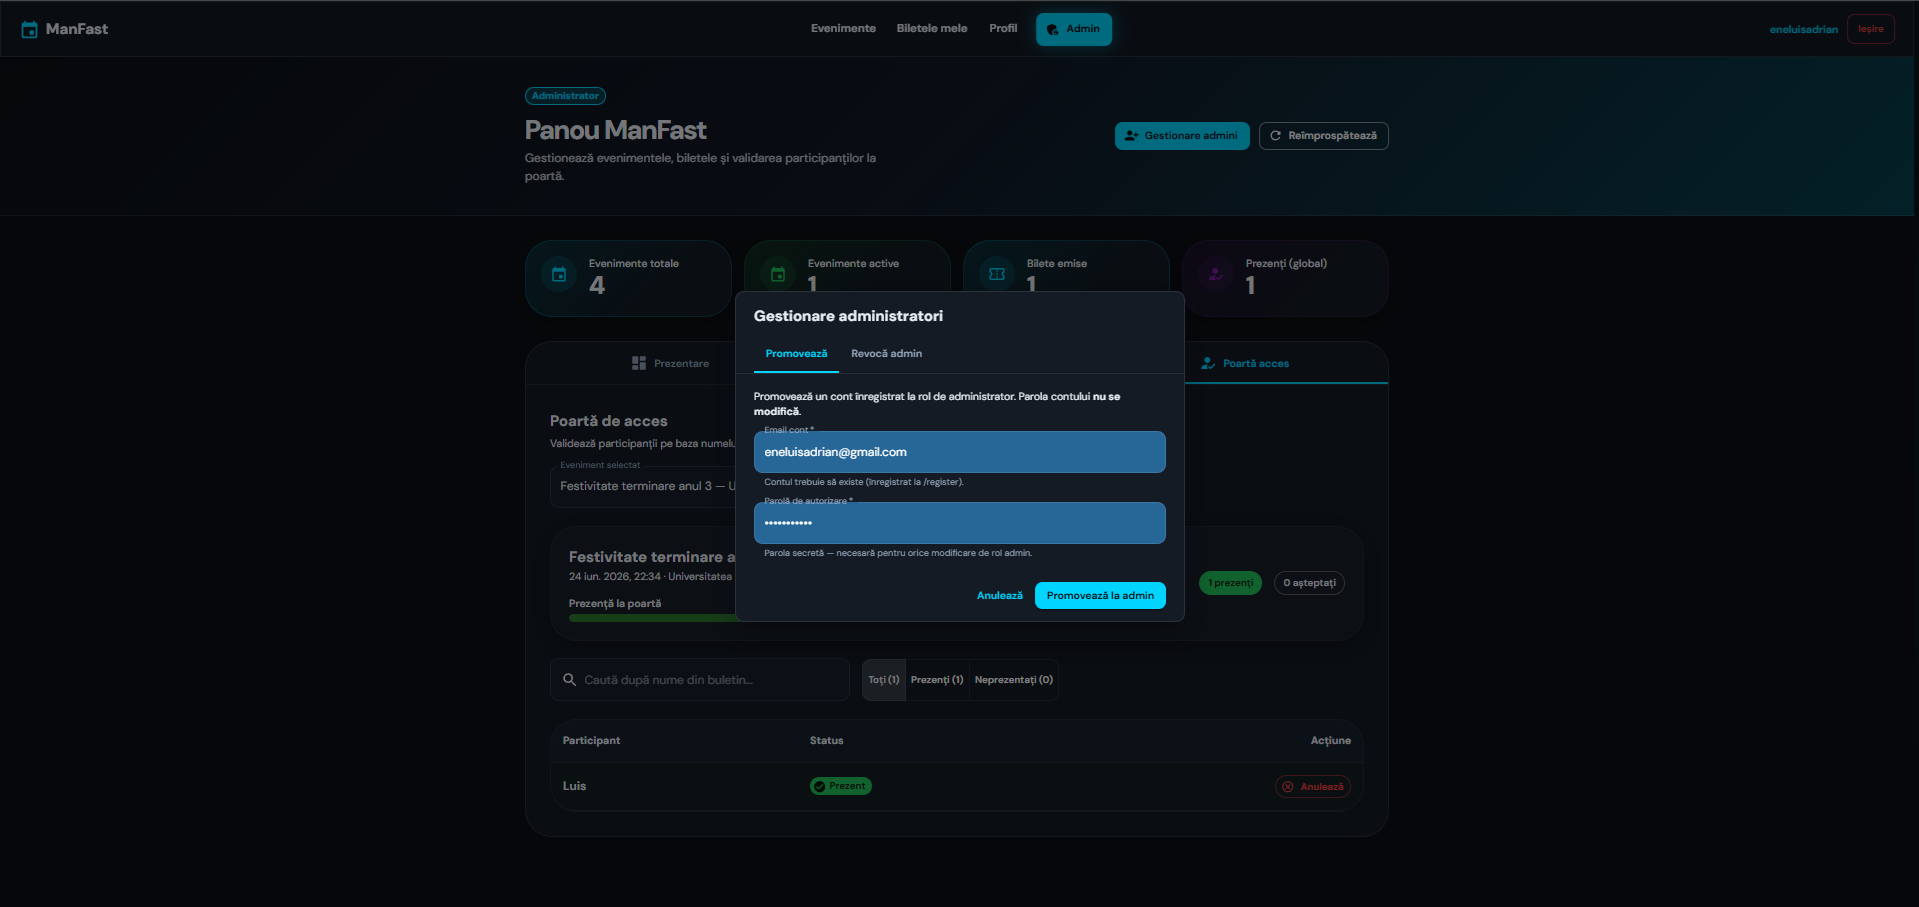
\includegraphics[width=1\textwidth]{Gestionare administratori.png}
	\caption{ Gestionare administratori}
	\label{fig:l2f1}
\end{figure}

\subsection{Conferin\c t\u a sau simpozion}

Pagina de detalii poate include \^in descriere: programul pe zile, lista speakerilor, link-uri c\u atre site-ul conferin\c tei. Imaginile \^inc\u arcate pot fi logo-ul evenimentului \c si fotografii din edi\c tii anterioare. Filtrele de pe Home permit g\u asirea conferin\c telor dintr-un anumit jude\c t sau dat\u a — util pentru participan\c ti care caut\u a evenimente academice regionale.

Formularul de cump\u arare bilet colecteaz\u a numele participantului (pentru ecuson sau list\u a oficial\u a). Dup\u a plat\u a, ,,Biletele mele`` afi\c seaz\u a evenimentul ca ,,viitor`` p\^an\u a la data desf\u a\c sur\u arii; ulterior trece automat \^in ,,trecute``.

\subsection{Concert sau spectacol}

Organizatorul pune accent pe elementele vizuale: mai multe imagini (arti\c sti, poster), descriere atractiv\u a, pre\c t \c si locuri limitate pentru a crea urgen\c t\u a. Utilizatorii pot cump\u ara bilete pentru mai multe persoane introduc\^and c\^ate un nume per c\^amp — potrivit pentru ie\c sirile \^in grup.

Navbar-ul \c si tema dark ofer\u a un aspect modern, aliniat la a\c stept\u arile publicului t\^an\u ar pentru evenimente culturale. Pagina de succes dup\u a Stripe confirm\u a achizi\c tia \c si \linebreak redirec\c tioneaz\u a spre bilete.

\subsection{Meeting, workshop sau seminar}

Pentru evenimente profesionale cu num\u ar mic de locuri, administratorul poate urm\u ari \^in timp real c\^ate locuri au r\u amas disponibile. Check-in-ul la intrare \^in sala de training confirm\u a prezen\c ta pentru certificat sau raport HR. Resetarea parolei \c si editarea profilului permit participan\c tilor s\u a-\c si men\c tin\u a contul pe termen lung, pentru evenimente recurente organizate de aceea\c si entitate.

\subsection{Eveniment sportiv (caz secundar)}

La competi\c tii, numele de pe bilet poate corespunde actului de identitate al sportivului. Admin-ul bifeaz\u a check-in la \^inregistrarea la concurs. Interfa\c ta nu afi\c seaz\u a distinc\c tii specifice (categorie greutate, gen), dar fluxul tehnic este identic — organizatorul completeaz\u a manual detaliile \^in titlu \c si descriere.

\subsection{Recomand\u ari pentru capturi de ecran (capitol 4)}

Pentru o documenta\c tie reprezentativ\u a, autorul poate crea \^in baza de date trei evenimente demonstrative:
\begin{itemize}
	\item ,,Conferin\c ta Na\c tional\u a Informatic\u a 2026`` — accent pe descriere lung\u a \c si dat\u a.
	\item ,,Concert Jazz Constan\c ta`` — accent pe galerie imagini.
	\item ,,Workshop React pentru \^Incep\u atori`` — accent pe locuri limitate (ex. 25).
\end{itemize}

Capturile din figurile 4.1--4.8 pot folosi oricare dintre aceste evenimente; important este ca textul lucr\u arii s\u a reflecte diversitatea cazurilor, nu doar un singur domeniu.


\subsection{Accesibilitate \c si public larg}

Indiferent de categorie, formularele respect\u a etichetare clar\u a, mesaje de eroare \^in rom\^an\u a \c si layout responsive. Participan\c tii mai pu\c tin obi\c snui\c ti cu tehnologia (ex. invita\c ti la conferin\c t\u a) beneficiaz\u a de flux liniar: Home $\rightarrow$ Detalii $\rightarrow$ Login/Register $\rightarrow$ Plat\u a $\rightarrow$ Bilete.

Aceste exemple completeaz\u a descrierea interfe\c tei \c si leag\u a capturile de ecran de cazuri reale de utilizare \^in domeniul conferin\c telor, concertelor \c si meeting-urilor. % OBLIGATORIU - Specializarea Informatica
\chapter{Concluzii}

\section{Rezultate ob\c tinute}

Lucrarea de licen\c t\u a a avut ca obiectiv dezvoltarea \textbf{aplica\c tiei web pentru organizarea \c si gestionarea evenimentelor}, orientate \^int\^ai spre conferin\c te, meeting-uri, concerte \c si evenimente culturale, cu suport complementar pentru competi\c tii sportive. Obiectivele propuse au fost atinse:

\begin{itemize}
	\item Aplica\c tie full-stack func\c tional\u a: React + Express + PostgreSQL.
	\item Autentificare complet\u a: \^inregistrare cu verificare email, login JWT, resetare parol\u a, profil, \c stergere cont.
	\item Listare \c si filtrare evenimente (nume, jude\c t, dat\u a).
	\item Pl\u a\c ti Stripe Checkout \^in RON; bilete nominale \c si ,,Biletele mele``.
	\item Panou admin: CRUD evenimente cu imagini, check-in, gestionare admini.
	\item Documentare: arhitectur\u a, ERD, UML, API REST, scenarii pe tipuri de evenimente.
\end{itemize}

Solu\c tia demonstreaz\u a integrarea unor tehnologii moderne \^intr-un produs coerent, adaptat contextului rom\^anesc (jude\c te, RON, email Brevo).


\section{Limit\u ari}

\begin{itemize}
	\item Lips\u a teste automate (unit/integration) \c si pipeline CI/CD.
	\item Promovarea primului administrator necesit\u a script SQL sau \texttt{promote-admin}.
	\item Emailurile depind de configurarea SMTP; \^in development, codurile pot ap\u area \^in consola backend.
	\item Confirmarea pl\u a\c tii se bazeaz\u a pe apel frontend \texttt{confirm-payment}; webhook Stripe ar \^imbun\u at\u a\c ti robuste\c tea.
	\item Un singur tip de pre\c t per eveniment — f\u ar\u a categorii VIP/standard sau locuri numerotate.
\end{itemize}

\section{Dezvolt\u ari viitoare}

Dezvoltarea aplica\c tiei poate fi continuat\u a prin abordarea limit\u arilor identificate \c si ad\u augarea de noi func\c tionalit\u a\c ti:

\begin{itemize}
	\item Categorii de bilete (conferin\c t\u a: early bird / regular; concert: VIP).
	\item Export participan\c ti CSV din panoul admin.
	\item Notific\u ari email la cump\u arare bilet reu\c sit\u a.
	\item Paginare evenimente \c si caching.
	\item Webhook Stripe pentru confirmare server-side.
	\item Teste automate \c si deploy containerizat (Docker).
	\item Aplica\c tie mobil\u a sau PWA pentru check-in offline.
	\item Module op\c tionale pentru evenimente sportive (echipe, program).
\end{itemize}

Aplica\c tia reprezint\u a o baz\u a solid\u a pentru extindere \^intr-un produs destinat organizatorilor de conferin\c te, concerte \c si meeting-uri, cu accent pe simplitate, securitate \c si experien\c ta utilizatorului. % OBLIGATORIU

\bibliographystyle{unsrt}
\setlength{\baselineskip}{\normalbaselineskip}
\setlength{\parskip}{0pt}
\bibliography{refs} % Fisierul continand bibliografia citata a lucrarii
\end{document}

